\documentclass[a4paper,10pt]{article}

% =========================
%        Packages
% =========================
\usepackage[left=2.5cm, right=2.5cm, top=3cm, bottom=3cm]{geometry}
\usepackage[UTF8]{ctex}
\usepackage{amsmath, amssymb}
\usepackage{booktabs}
\usepackage{array}
\usepackage{graphicx}
\usepackage{float}
\usepackage{hyperref}
\usepackage{xcolor}
\usepackage{listings}
\usepackage{listings}
\usepackage{threeparttable}
\usepackage{multirow} 

% ── 数学与表格 ────────────────────────────────────────────────────────
\usepackage{amsmath, amssymb, booktabs, multirow, makecell, array}
\usepackage{longtable}
\usepackage{tabularx}

% ── 图形 ─────────────────────────────────────────────────────────────
\usepackage{graphicx}
\usepackage{float}
\usepackage{caption}
\usepackage{subcaption}

% ── 颜色与链接 ────────────────────────────────────────────────────────
\usepackage{xcolor}
\usepackage[colorlinks=true, linkcolor=blue, citecolor=blue]{hyperref}

% ── 参考文献 ─────────────────────────────────────────────────────────
\usepackage{natbib}

% ── 其他 ─────────────────────────────────────────────────────────────
\usepackage{enumitem}
\usepackage{footnote}

% ── 自定义命令 ────────────────────────────────────────────────────────
\newcommand{\figref}[2]{\textit{（第#1格第#2幅图）}}
\newcommand{\pvalue}[1]{\(p = #1\)}
\newcommand{\tstat}[1]{\(t = #1\)}


% --- code block style ---
\lstset{
    language=Python,
    basicstyle=\ttfamily\footnotesize,
    keywordstyle=\color{blue},
    stringstyle=\color{red},
    commentstyle=\color{green!50!black},
    numbers=left,
    numberstyle=\tiny\color{gray},
    stepnumber=1,
    breaklines=true,
    frame=single,
    backgroundcolor=\color{gray!5},
    showstringspaces=false,
    captionpos=b,
    tabsize=4
}

% =========================
%        Document
% =========================
\begin{document}

% =========================
%        Cover
% =========================
\begin{center}
    \vspace*{1cm}
    {\Huge ZO-1 Capstone 双周报 5}
    
    \vspace{2.2cm}
    {\Large April 12， 2026}
    
    \vspace{1.2cm}
    \renewcommand{\arraystretch}{1.5}
    \begin{tabular}{@{} >{\bfseries}l l @{}}
        \toprule[1.5pt]
        项目企业 & 中欧瑞博 \\
        项目名称 & 股东回报因子探索：考虑净回购的股息率 + 因子 \\
        学生姓名 & 沈可涵 (123090483), 蒋之伟 (123090233), 杨衍韬 (123090731) \\
        报告周期 & 2026 年 3 月 30 日至 2026 年 4 月 12 日 \\
        提交日期 & 2026 年 4 月 12 日 \\
        \bottomrule[1.5pt]
    \end{tabular}
\end{center}

\newpage
\tableofcontents
\newpage

% =========================
%        Main Text
% =========================

\section{大纲与本期更新摘要}

\subsection{整体研究大纲}

本文研究主要分为两个部分：

\begin{enumerate}
    \item \textbf{回购行为定价研究（日频）}
    \begin{itemize}
        \item 数据构建与样本筛选（流动性与回购活跃度）
        \item 回购因子构建（滚动规模与归一化指标）
        \item 预测能力检验（IC 与多空组合）
        \item 因子增强（动态变化、事件交互、残差化）
        \item 定价机制分析（事件驱动与延迟定价）
        \item 稳健性检验（样本外与样本选择偏差）
        \item 多期收益与信号时效性分析
    \end{itemize}
    
    \item \textbf{现金流质量因子研究（月频）}
    \begin{itemize}
        \item 八分组与动态四分组框架
        \item 双重排序方法与局限性分析
        \item 单因子检验（CFO Coverage / Yield / TTM）
        \item 净股东回报收益率（NPY）分析
        \item 方法论局限与可交易性讨论
    \end{itemize}
\end{enumerate}

\subsection{本期更新摘要}

本期研究重点围绕回购行为定价机制深化及现金流质量因子扩展验证展开，主要结论如下：

\begin{itemize}
    \item \textbf{回购因子方面}：
    \begin{itemize}
        \item 回购规模具有稳定预测能力，且\textbf{绝对规模优于归一化指标}；
        \item 引入事件交互后，IC 显著提升，验证\textbf{事件驱动是核心机制}；
        \item 回购信号在中长期 horizon 下持续增强，表明存在\textbf{延迟定价效应}；
        \item 样本筛选显著增强因子表现，但引入\textbf{事件富集的条件性 alpha}。
    \end{itemize}
    
    \item \textbf{现金流因子方面}：
    \begin{itemize}
        \item 八分组与四分组框架均具有显著截面预测能力；
        \item 双重排序因样本稀疏失效，属于\textbf{方法约束而非信号失效}；
        \item CFO 类因子均具有显著 IC，但仅在等权下有效，市值加权后信号消失；
        \item NPY 因子本质来源于\textbf{是否股权融资}这一离散维度，而非连续排序能力。
    \end{itemize}
    
    \item \textbf{核心结论}：
    \begin{itemize}
        \item 回购与现金流信号均呈现\textbf{事件驱动 + 条件性 alpha}特征；
        \item 因子有效性高度依赖样本选择与市值结构；
        \item 当前结果更适用于解释经济机制，\textbf{尚不具备直接可交易性}。
    \end{itemize}
\end{itemize}


\section{回购信号的深入实证分析 与 事件驱动定价延时机制研究}


\subsection{数据构建与样本筛选}

\subsubsection{原始数据处理与收益构造}

本文所使用的数据来源于包含公司回购行为标记的日频股票数据集。首先，对原始数据进行预处理，包括时间序列排序与变量构造。具体而言，对每只股票按照交易日期进行升序排序，并将日期字段统一转换为标准时间格式。

在收益率构造方面，本文采用前瞻收益（forward return）作为预测目标变量。对于股票 $i$ 在时点 $t$，其下一期收益定义为：
\begin{equation}
r_{i,t+1} = \frac{P_{i,t+1}}{P_{i,t}} - 1
\end{equation}
其中，$P_{i,t}$ 表示股票 $i$ 在时点 $t$ 的复权收盘价（AdjClose）。该收益率定义能够较好反映基于当前信息进行预测的实际投资回报。

此外，为便于后续分析，进一步提取年份变量：
\begin{equation}
\text{year}_t = \text{Year}(\text{date}_t)
\end{equation}

\subsubsection{流动性筛选}

考虑到低流动性股票可能存在价格失真、交易冲击较大等问题，本文首先对样本进行流动性筛选。具体方法如下：

对于每只股票 $i$ 在年份 $y$，计算其年度平均成交额：
\begin{equation}
\text{liq}_{i,y} = \frac{1}{N_{i,y}} \sum_{t \in y} \text{amount}_{i,t}
\end{equation}
其中，$\text{amount}_{i,t}$ 表示股票 $i$ 在时点 $t$ 的成交额，$N_{i,y}$ 为该股票在年份 $y$ 的交易日数量。

随后，在每一年内部，对所有股票的流动性进行排序，并计算其中位数阈值：
\begin{equation}
\text{threshold}_y = \text{Median} \left( \{ \text{liq}_{i,y} \}_{i \in \mathcal{S}_y} \right)
\end{equation}

仅保留满足以下条件的股票进入后续分析：
\begin{equation}
\text{liq}_{i,y} \geq \text{threshold}_y
\end{equation}

该筛选过程能够有效剔除流动性较差的股票，提高实证结果的稳定性与可交易性。

\subsubsection{回购行为活跃度筛选}

在流动性筛选基础上，本文进一步基于公司回购行为的活跃程度进行样本筛选。具体步骤如下：

首先，对每只股票统计其在样本期内的总交易日数与发生回购行为的交易日数：
\begin{align}
N_i^{\text{total}} &= \text{Total trading days of stock } i \\
N_i^{\text{bb}} &= \text{Number of days with buyback activity}
\end{align}

据此构造回购行为占比指标：
\begin{equation}
\text{ratio}_i = \frac{N_i^{\text{bb}}}{N_i^{\text{total}}}
\end{equation}

为了刻画回购行为在整体市场中的分布特征，进一步对该比例进行归一化处理，定义权重：
\begin{equation}
w_i = \frac{\text{ratio}_i}{\sum_{j} \text{ratio}_j}
\end{equation}

并计算其累计权重：
\begin{equation}
\text{cum\_weight}_i = \sum_{j \leq i} w_j
\end{equation}
其中股票按照 $\text{ratio}_i$ 从高到低排序。

最终，选取满足以下条件的股票作为研究样本：
\begin{equation}
\text{cum\_weight}_i \leq 0.8 \quad \text{and} \quad N_i^{\text{total}} > 100
\end{equation}

该筛选方法的直观含义是：保留回购行为最活跃的前 $80\%$ 股票（按加权分布），同时剔除交易记录过少的个股，以避免小样本带来的估计偏差。

\subsubsection{最终样本构建}

在完成上述筛选后，本文最终构建得到研究样本集合：
\begin{equation}
\mathcal{S}^{\text{final}} = \left\{ i \mid i \in \text{Top buyback stocks and high liquidity set} \right\}
\end{equation}

并基于该股票池提取对应的日频数据，形成后续因子构建与预测分析的基础数据集。

通过上述多重筛选机制，本文确保所使用的数据同时具备良好的流动性与足够的回购行为观测，从而提高实证结果的经济解释力与稳健性。





\subsection{回购因子构建与预测能力检验}

\subsubsection{回购规模的滚动构建}

在完成样本筛选后，本文进一步构建基于公司回购行为的连续型因子。考虑到回购行为具有显著的时间累积特征，本文采用滚动窗口方法刻画不同时间尺度下的回购强度。

首先，将原始回购金额缺失值填充为零：
\begin{equation}
\widetilde{\text{BB}}_{i,t} = 
\begin{cases}
\text{BB}_{i,t}, & \text{if observed} \\
0, & \text{otherwise}
\end{cases}
\end{equation}

在此基础上，定义不同时间窗口下的滚动回购金额：
\begin{align}
\text{BB}^{(1Y)}_{i,t} &= \sum_{s=t-251}^{t} \widetilde{\text{BB}}_{i,s} \\
\text{BB}^{(2Y)}_{i,t} &= \sum_{s=t-503}^{t} \widetilde{\text{BB}}_{i,s} \\
\text{BB}^{(3Y)}_{i,t} &= \sum_{s=t-755}^{t} \widetilde{\text{BB}}_{i,s}
\end{align}

其中，1年、2年和3年的窗口长度分别取252、504和756个交易日。

\subsubsection{回购归一化因子构建}

为了消除公司规模差异带来的影响，本文从两个角度对回购金额进行归一化处理。

\paragraph{（1）基于市值的回购收益率（Buyback Yield）}

定义回购收益率为滚动回购金额与当前市值之比：
\begin{equation}
\text{BY}^{(k)}_{i,t} = \frac{\text{BB}^{(k)}_{i,t}}{\text{MKTCP}_{i,t}}, \quad k \in \{1Y, 2Y, 3Y\}
\end{equation}

其中，市值定义为：
\begin{equation}
\text{MKTCP}_{i,t} = P_{i,t} \times \text{Shares}_{i,t}
\end{equation}

该指标刻画了公司通过回购向股东“返还资本”的相对强度。

\paragraph{（2）基于价格的回购强度指标}

进一步构造另一类归一化指标，将回购金额与股票价格进行对比：
\begin{equation}
\text{BS}^{(k)}_{i,t} = \frac{\text{BB}^{(k)}_{i,t}}{P_{i,t}}, \quad k \in \{1Y, 2Y, 3Y\}
\end{equation}

该指标从“潜在回购股份数量”的角度刻画回购力度。

\subsubsection{因子预测能力检验方法}

本文采用信息系数（Information Coefficient, IC）衡量因子的预测能力。具体而言，在每个交易日 $t$，计算因子值与下一期收益的截面 Spearman 相关系数：
\begin{equation}
\text{IC}_t = \text{corr}_{\text{Spearman}} \left( f_{i,t}, r_{i,t+1} \right)
\end{equation}

并对时间序列上的 IC 进行统计汇总：
\begin{align}
\text{IC}_{\text{mean}} &= \frac{1}{T} \sum_{t=1}^{T} \text{IC}_t \\
\text{IC}_{\text{t-stat}} &= \frac{\text{IC}_{\text{mean}}}{\sigma(\text{IC})} \sqrt{T}
\end{align}

其中 $\sigma(\text{IC})$ 表示 IC 的时间序列标准差。

\subsubsection{实证结果分析}

表 \ref{tab:bb_ic} 报告了不同回购因子的 IC 统计结果。

\begin{table}[H]
\centering
\caption{回购因子 IC 统计结果}
\label{tab:bb_ic}
\begin{tabular}{lcccc}
\toprule
因子 & IC Mean & IC Std & t-stat & N \\
\midrule
Buyback\_3Y & 0.0134 & 0.2178 & 3.17 & 2643 \\
Buyback\_2Y & 0.0131 & 0.2173 & 3.09 & 2643 \\
Buyback\_1Y & 0.0123 & 0.2195 & 2.89 & 2643 \\
BS\_1Y      & 0.0058 & 0.2094 & 1.42 & 2643 \\
BS\_3Y      & 0.0055 & 0.2093 & 1.36 & 2643 \\
BS\_2Y      & 0.0054 & 0.2075 & 1.34 & 2643 \\
BY\_1Y      & 0.0028 & 0.2089 & 0.69 & 2643 \\
BY\_3Y      & 0.0028 & 0.2086 & 0.68 & 2643 \\
BY\_2Y      & 0.0025 & 0.2062 & 0.63 & 2643 \\
\bottomrule
\end{tabular}
\end{table}

从结果可以得到以下几点重要结论：

\begin{itemize}
    \item \textbf{回购规模本身具有显著预测能力}：滚动回购金额（Buyback）在所有因子中表现最优，其 IC 均值约为 $0.012 \sim 0.013$，且 t-stat 超过 2.8，具有统计显著性。
    
    \item \textbf{时间窗口越长，信号越稳定}：3 年滚动窗口的表现略优于 1 年窗口，说明回购行为具有长期信息含量，而非短期噪声。
    
    \item \textbf{归一化处理削弱了预测能力}：无论是基于市值的 Buyback Yield，还是基于价格的回购强度指标，其 IC 均明显低于原始回购金额。这表明规模信息本身可能包含重要的横截面信号。
    
    \item \textbf{回购行为具有“规模驱动”特征}：结果表明，大规模回购公司往往具有更强的未来收益表现，而简单的比例标准化可能削弱这一信息。
\end{itemize}

总体而言，回购行为作为一种公司主动资本配置决策，能够提供有效的横截面定价信息，其中绝对规模比相对比例更具预测价值。




\subsection{回购因子的增强构建与机制扩展}

在基础回购因子构建的基础上，本文进一步从数据处理、动态信息提取以及事件交互等多个维度对因子进行增强，以挖掘更深层次的定价信息。

\subsubsection{分布调整与标准化处理}

考虑到回购金额分布通常具有明显的长尾特征，直接使用原始变量可能受到极端值的干扰。因此，本文首先在截面上对因子进行缩尾处理（winsorization）。对于任意因子 $x_{i,t}$，在每个交易日 $t$ 上进行如下处理：
\begin{equation}
x^{\text{win}}_{i,t} = \min\left( \max\left(x_{i,t}, Q_{1\%}(t)\right), Q_{99\%}(t) \right)
\end{equation}

在此基础上，为进一步缓解分布偏态问题，对变量进行对数变换：
\begin{equation}
x^{\log}_{i,t} = \log(1 + x_{i,t})
\end{equation}

同时，本文采用截面排序标准化方法，将因子映射至 $[-0.5, 0.5]$ 区间：
\begin{equation}
x^{\text{rank}}_{i,t} = \text{rank}(x_{i,t}) - 0.5
\end{equation}

上述处理能够显著提高因子的稳健性与可比性。

\subsubsection{动态变化与相对结构因子}

除静态回购规模外，本文进一步构造反映回购行为动态变化的因子。具体包括：

\paragraph{（1）回购加速度指标}
\begin{align}
\Delta \text{BB}^{(1Y)}_{i,t} &= \text{BB}^{(1Y)}_{i,t} - \frac{1}{2}\text{BB}^{(2Y)}_{i,t} \\
\Delta \text{BB}^{(2Y)}_{i,t} &= \text{BB}^{(2Y)}_{i,t} - \frac{2}{3}\text{BB}^{(3Y)}_{i,t}
\end{align}

该类指标刻画公司回购行为是否呈现“加速”趋势。

\paragraph{（2）回购结构比例指标}
\begin{align}
\text{Ratio}_{1/2} &= \frac{\text{BB}^{(1Y)}_{i,t}}{\text{BB}^{(2Y)}_{i,t}} \\
\text{Ratio}_{1/3} &= \frac{\text{BB}^{(1Y)}_{i,t}}{\text{BB}^{(3Y)}_{i,t}}
\end{align}

该类指标用于刻画短期回购相对于长期回购的占比，从而反映公司资本配置的时序结构。

\subsubsection{事件交互因子构建}

为了捕捉回购行为与信息披露事件之间的交互效应，本文构造了回购规模与事件变量的交互项。设事件指示变量为 $D_{i,t}$，则定义：
\begin{equation}
\text{BB}^{(3Y)}_{i,t} \times D_{i,t}
\end{equation}

其中事件变量包括：回购执行公告、次日公告、完成公告以及是否存在任一回购事件等。此外，还进一步引入回购公告数量作为连续型信息强度变量：
\begin{equation}
\text{BB}^{(3Y)}_{i,t} \times N^{\text{ann}}_{i,t}
\end{equation}

该类因子刻画了“回购规模 $\times$ 信息确认强度”的交互机制。

\subsubsection{去规模与残差化处理}

为进一步区分回购行为中的“纯规模效应”与“超额信息含量”，本文采用截面回归的方法对回购因子进行残差化处理。

具体而言，在每个交易日 $t$ 上进行如下回归：
\begin{equation}
\log(\text{BB}^{(3Y)}_{i,t}) = \alpha_t + \beta_t \log(\text{MKTCP}_{i,t}) + \gamma_t \log(P_{i,t}) + \epsilon_{i,t}
\end{equation}

并将残差项 $\epsilon_{i,t}$ 作为新的因子：
\begin{equation}
\text{BB}^{\text{resid}}_{i,t} = \epsilon_{i,t}
\end{equation}

该处理方法能够有效剥离公司规模与价格水平的影响，从而识别回购行为中的“异常成分”。

\subsubsection{增强因子的实证结果分析}

表 \ref{tab:enhanced_ic} 展示了增强后因子的 IC 表现。

\begin{table}[H]
\centering
\caption{增强回购因子 IC 统计结果（部分）}
\label{tab:enhanced_ic}
\begin{tabular}{lccc}
\toprule
因子 & IC Mean & t-stat & 说明 \\
\midrule
BB\_3Y $\times$ NextDay & 0.0387 & 7.77 & 事件驱动增强 \\
BB\_3Y $\times$ Announcement & 0.0374 & 7.55 & 信息强度增强 \\
BB\_3Y $\times$ Execution & 0.0364 & 7.36 & 执行确认效应 \\
BB\_3Y $\times$ AnyEvent & 0.0360 & 7.27 & 广义事件效应 \\
BB\_3Y（基础） & 0.0134 & 3.17 & 基准因子 \\
BB\_3Y（残差） & 0.0070 & 1.63 & 去规模后信号 \\
\bottomrule
\end{tabular}
\end{table}

可以得到如下关键结论：

\begin{itemize}
    \item \textbf{事件交互显著增强预测能力}：所有“回购 $\times$ 事件”类因子的 IC 均显著高于基础因子，提升幅度接近 2-3 倍，表明市场对“已确认回购行为”的反应更为强烈。
    
    \item \textbf{信息披露具有放大效应}：回购公告数量与回购规模的交互项表现优异，说明信息频率能够强化回购信号。
    
    \item \textbf{动态因子贡献有限但稳定}：回购加速度与比例类因子虽有一定预测能力，但显著性较弱，表明市场更关注绝对规模而非变化趋势。
    
    \item \textbf{去规模后信号明显减弱}：残差化后的因子 IC 明显下降，进一步验证了回购信号中“规模效应”的重要性。
\end{itemize}

综上，回购行为的预测能力不仅来源于其规模本身，更依赖于信息披露的时点与强度，体现出典型的“事件驱动型定价机制”。




\subsection{回测结果与事件驱动机制验证}

\subsubsection{多空组合回测结果}

在因子预测能力检验的基础上，本文进一步通过构建多空组合（long-short portfolio）评估因子的实际投资价值。具体而言，在每个交易日 $t$，根据因子值对股票进行排序，并划分为 $q=5$ 个分位组，构造多空组合收益：
\begin{equation}
\text{LS}_t = \mathbb{E}[r_{i,t+1} \mid i \in \text{Top}] - \mathbb{E}[r_{i,t+1} \mid i \in \text{Bottom}]
\end{equation}

其中 Top 和 Bottom 分别表示因子值最高与最低的分组。

表 \ref{tab:ls_result} 报告了主要因子的回测结果。

\begin{table}[H]
\centering
\caption{多空组合回测结果（部分）}
\label{tab:ls_result}
\begin{tabular}{lccc}
\toprule
因子 & Mean Daily LS & t-stat & N \\
\midrule
Log(BB 1Y / 3Y) Rank & 0.000789 & 2.40 & 2522 \\
Log Residual (Size+Price) & 0.000527 & 1.45 & 2208 \\
BB3Y $\times$ Execution & 0.000310 & 0.56 & 1030 \\
Residual Size Only & 0.000271 & 0.70 & 2208 \\
Log BB3Y Rank & 0.000225 & 0.66 & 2629 \\
Raw BB3Y & 0.000225 & 0.66 & 2629 \\
\bottomrule
\end{tabular}
\end{table}

结果表明：

\begin{itemize}
    \item \textbf{因子在投资层面具有一定收益能力}：部分增强因子（如回购结构比例）在多空组合中表现出显著正收益，t-stat 超过 2。
    
    \item \textbf{IC 与收益并非完全一致}：尽管事件交互因子在 IC 层面表现优异，但在多空组合中未完全转化为稳定收益，说明预测能力与可交易性之间存在差异。
    
    \item \textbf{结构性信息更具交易价值}：相较于绝对规模，回购结构（如短期/长期比例）在组合收益中表现更优。
\end{itemize}

\subsubsection{事件变量的独立预测能力}

为进一步分析回购行为的来源，本文首先检验事件变量自身是否具备预测能力。结果显示：

\begin{itemize}
    \item Next-day 公告、执行公告等事件变量均具有较高 IC（约 $0.037 \sim 0.039$）；
    \item t-stat 均超过 7，具有极强统计显著性。
\end{itemize}

该结果表明，市场对回购信息披露本身存在显著反应，支持“事件驱动”假说。

\subsubsection{条件分析：回购在事件发生后的有效性}

进一步地，本文在事件发生子样本中检验回购因子的有效性。

在 $\text{hit\_nextday}=1$ 和 $\text{hit\_execution}=1$ 的子样本中，回购因子的 IC 表现如下：
\begin{itemize}
    \item 回购因子 IC 转为负值（约 $-0.02$）；
    \item t-stat 不显著。
\end{itemize}

这一结果表明：

\begin{equation}
\text{Predictive Power of Buyback} \mid \text{Event Occurred} \approx 0
\end{equation}

即，一旦事件信息被市场观测，回购规模本身不再提供额外预测能力。

\subsubsection{残差化检验：是否存在独立信息}

为了进一步验证回购与事件之间的信息关系，本文对交互因子进行残差化处理：

\begin{equation}
(\text{BB} \times D)^{\text{resid}} = (\text{BB} \times D) - \beta D
\end{equation}

实证结果显示：
\begin{itemize}
    \item 残差化后的因子 IC 接近 0；
    \item t-stat 不显著。
\end{itemize}

该结果说明：

\begin{equation}
\text{Alpha}_{\text{BB} \times D} \approx \text{Alpha}_{D}
\end{equation}

即交互项的预测能力主要来源于事件变量本身，而非回购规模的独立贡献。

\subsubsection{时间稳定性分析}

最后，本文从时间维度考察因子的稳定性。将样本按年份划分，计算年度 IC，结果表明：

\begin{itemize}
    \item 因子在大多数年份均保持正 IC（约 $0.03 \sim 0.07$）；
    \item 在个别年份（如 2019、2025）出现短暂失效；
    \item 整体来看，信号具有较强的跨期稳定性。
\end{itemize}

\subsubsection{小结：回购行为的定价机制}

综合上述结果，可以得到一个清晰的机制解释：

\begin{enumerate}
    \item \textbf{回购规模本身包含信息}：在无事件条件下，回购规模具有一定预测能力；
    
    \item \textbf{事件是核心驱动因素}：信息披露显著增强信号强度；
    
    \item \textbf{信息一旦公开即被定价}：在事件发生后，回购因子的预测能力消失；
    
    \item \textbf{交互项本质上是事件代理变量}：其 alpha 来源于事件而非回购本身。
\end{enumerate}

因此，本文认为回购行为的定价机制具有典型的“信息驱动 + 事件触发”特征，而非简单的基本面因子效应。



\subsection{样本外检验与样本选择偏差分析}

\subsubsection{样本外（Out-of-Sample）预测能力验证}

为了检验因子是否存在过拟合问题，本文采用时间序列划分方法进行样本外（Out-of-Sample, OOS）检验。具体而言，将样本按照时间排序，并以 $70\%$ 的时间段作为训练集，其余 $30\%$ 作为测试集。

在训练集与测试集中分别计算因子的 IC 均值与 t 统计量。结果如表 \ref{tab:oos_result} 所示。

\begin{table}[H]
\centering
\caption{样本内与样本外 IC 对比}
\label{tab:oos_result}
\begin{tabular}{lcccc}
\toprule
因子 & Train IC & Test IC & Train t-stat & Test t-stat \\
\midrule
BB3Y $\times$ NextDay & 0.0411 & 0.0346 & 6.87 & 3.94 \\
BB3Y $\times$ Execution & 0.0380 & 0.0336 & 6.40 & 3.83 \\
BB3Y & 0.0059 & 0.0311 & 1.18 & 3.87 \\
\bottomrule
\end{tabular}
\end{table}

可以观察到：

\begin{itemize}
    \item \textbf{事件交互因子在样本外仍然显著}：尽管预测能力有所衰减，但 Test IC 仍维持在较高水平（约 0.03），表明因子具有较强的泛化能力；
    
    \item \textbf{基础回购因子在样本外表现提升}：原始回购规模在测试集中的 IC 明显高于训练集，可能反映出市场结构变化或样本划分带来的差异；
    
    \item \textbf{不存在明显过拟合现象}：整体来看，训练集与测试集之间的性能差异较为平滑，说明模型稳健性较强。
\end{itemize}

\subsubsection{原始样本与筛选样本的对比分析}

为进一步检验样本筛选对结果的影响，本文在原始数据（未进行流动性与回购筛选）上重新评估事件变量的预测能力。

结果显示，在原始样本中：

\begin{itemize}
    \item 事件变量的 IC 均值约为 $0.013 \sim 0.014$；
    \item t-stat 显著，但明显低于筛选样本中的结果（约 $0.037$）。
\end{itemize}

进一步比较筛选前后 IC 提升幅度：
\begin{equation}
\Delta \text{IC} \approx 0.02 \sim 0.03
\end{equation}

该结果表明，样本筛选显著增强了因子的预测能力。

\subsubsection{样本选择机制分析}

为了理解上述现象，本文进一步分析原始样本与筛选样本之间的结构差异。结果表明：

\begin{itemize}
    \item 筛选样本中事件发生概率显著提高；
    \item 例如，Next-day 事件发生率由约 2.4\% 提升至 17.8\%；
    \item 回购公告数量等指标也呈现类似上升趋势。
\end{itemize}

这意味着筛选过程实际上构建了一个“事件富集”（event-enriched）的样本空间。

\subsubsection{样本选择偏差的经济含义}

上述结果揭示了一个重要现象：

\begin{equation}
\text{Alpha}_{\text{Filtered}} > \text{Alpha}_{\text{Full Sample}}
\end{equation}

其原因并非因子本身更强，而是由于：

\begin{enumerate}
    \item \textbf{筛选过程提高了信号密度}：更多包含回购事件的股票进入样本；
    
    \item \textbf{降低了噪声比例}：剔除了无回购或低流动性股票；
    
    \item \textbf{增强了事件驱动特征}：使得因子更接近“条件 alpha”（conditional alpha）。
\end{enumerate}

因此，筛选后的结果更接近于：
\begin{equation}
\text{Alpha} \mid \text{High Event Probability}
\end{equation}

而非无条件的横截面预测能力。

\subsubsection{小结：稳健性与外推能力}

综合样本外检验与样本对比分析，本文得到如下结论：

\begin{itemize}
    \item 因子在样本外仍具有显著预测能力，具有一定泛化性；
    
    \item 样本筛选显著增强了因子表现，但同时引入了“事件选择偏差”；
    
    \item 回购因子的有效性在很大程度上依赖于样本中事件的出现频率；
    
    \item 因此，其预测能力更应被理解为一种“条件性 alpha”，而非普适因子。
\end{itemize}

这一发现对于因子构建与实证研究具有重要启示：在评估因子性能时，必须充分考虑样本选择机制对结果的影响。




\subsection{多期收益分析与信号时效性研究}

\subsubsection{多期前瞻收益构建}

为了进一步分析回购事件对未来收益的影响路径，本文构建了多期前瞻收益。对于股票 $i$ 在时点 $t$，定义 $h$ 日前瞻收益为：
\begin{equation}
r_{i,t+h} = \frac{P_{i,t+h}}{P_{i,t}} - 1
\end{equation}

其中，$P_{i,t}$ 表示股票 $i$ 在时点 $t$ 的复权收盘价，$h$ 表示预测期限。本文首先考察短中期 horizon（如 1--60 个交易日），随后将预测窗口进一步延长，以检验事件信号是否具有更长时间尺度上的持续影响。

\subsubsection{跨期 IC 计算方法}

在每一个预测窗口 $h$ 下，计算事件因子与对应前瞻收益之间的截面 Spearman 相关性：
\begin{equation}
\text{IC}^{(h)}_t = \mathrm{corr}_{\mathrm{Spearman}}\left(f_{i,t}, r_{i,t+h}\right)
\end{equation}

并进一步对时间序列上的日度 IC 求均值，得到该 horizon 下的整体预测能力：
\begin{equation}
\overline{\text{IC}}^{(h)} = \frac{1}{T}\sum_{t=1}^{T}\text{IC}^{(h)}_t
\end{equation}

本文重点考察三类事件变量：次日公告事件（hit\_nextday）、执行公告事件（hit\_execution）以及综合事件指示变量（has\_any\_event）。

\subsubsection{不同预测窗口下的实证结果}

图 \ref{fig:event_ic_horizon_60} 和图 \ref{fig:event_ic_horizon_long} 分别展示了事件因子在短中期 horizon 与扩展 horizon 下的 IC 变化趋势。

\begin{figure}[H]
\centering
\begin{subfigure}[b]{0.48\textwidth}
    \centering
    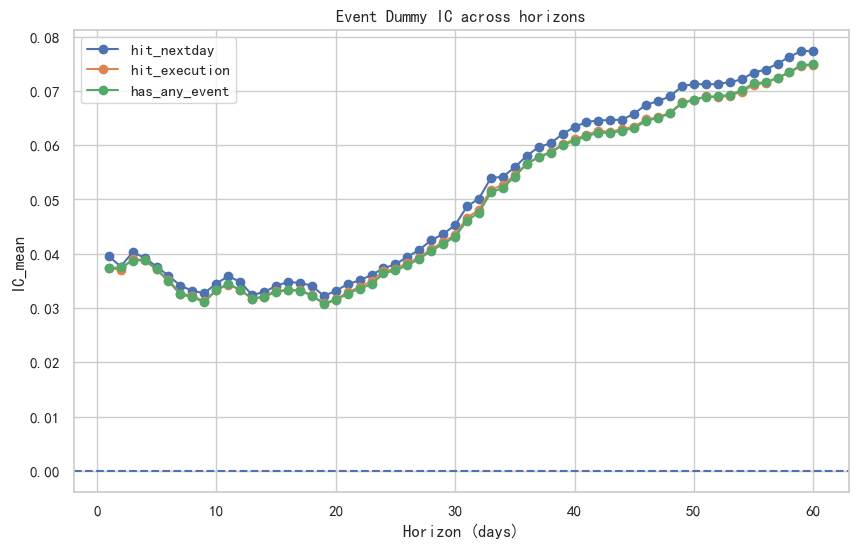
\includegraphics[width=\textwidth]{event_ic_horizon_60.png}
    \caption{短中期预测窗口下的 IC 变化（1--60 日）}
    \label{fig:event_ic_horizon_60}
\end{subfigure}
\hfill
\begin{subfigure}[b]{0.48\textwidth}
    \centering
    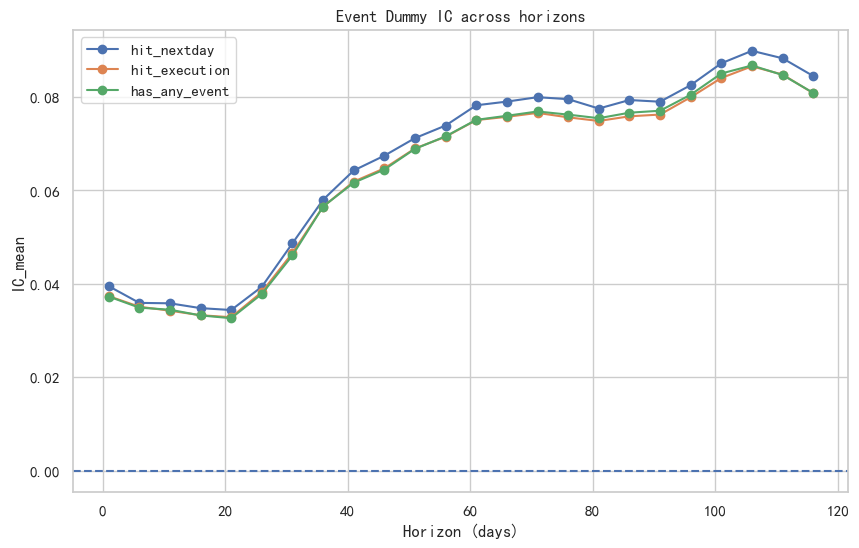
\includegraphics[width=\textwidth]{event_ic_horizon_long.png}
    \caption{扩展预测窗口下的 IC 变化}
    \label{fig:event_ic_horizon_long}
\end{subfigure}
\caption{事件因子在不同预测窗口下的 IC 变化趋势}
\label{fig:event_ic_horizon_all}
\end{figure}

从两张图中可以得到以下几点结论。

首先，在较短 horizon 下，事件变量已经表现出稳定为正的预测能力。无论是 hit\_nextday、hit\_execution 还是 has\_any\_event，其 IC 在短期内均显著高于 0，说明回购相关事件在发生当期即包含明确的横截面定价信息。

其次，在 1--60 个交易日的区间内，事件信号并未随 horizon 增加而衰减，反而整体呈现逐步上升趋势。尤其是在大约 30 日之后，三类事件变量的 IC 开始更明显地抬升，表明市场并未在极短时间内一次性完成对回购信息的定价，而是存在持续的信息扩散与价格修正过程。

进一步地，当预测窗口被扩展到更长 horizon 后，这一结论依然成立。扩展图显示，IC 在更长区间内继续维持在较高水平，并在约 100 个交易日前后达到局部高点。以 hit\_nextday 为例，其 IC 均值在长 horizon 下上升至约 0.09 左右；hit\_execution 与 has\_any\_event 的走势也高度一致，仅在数值上略低于 hit\_nextday。整体来看，三条曲线保持较强的同步性，说明不同事件定义所反映的本质信息较为一致。

最后，从长 horizon 末端的表现来看，IC 虽然出现小幅波动，但并未明显回落至接近 0 的水平。这表明回购事件所携带的信息并非仅仅对应短期交易冲击，而更可能反映公司基本面改善、管理层估值信号或资本配置质量等长期信息，因此其影响具有较强的持续性。

\subsubsection{经济解释：延迟定价与长期信息释放}

上述结果表明，回购事件的价格影响机制并不符合“即时完全反应”的模式，而更接近于一种延迟定价过程。形式上可以表示为：
\begin{equation}
\text{Price Adjustment to Buyback Event} \neq \text{Instantaneous}
\end{equation}

这种现象可能来源于以下几个方面。

第一，回购公告本身具有较强的信息复杂性。市场不仅需要识别事件是否发生，还需要进一步判断其背后所隐含的管理层信号、公司现金流状况以及估值修复空间，因此价格反应往往分阶段完成。

第二，不同类型投资者对回购事件的反应速度并不一致。短线交易者可能首先捕捉公告本身，而中长期投资者则更关注事件背后的基本面含义，这会导致价格在较长时间内持续调整。

第三，部分机构投资者在仓位调整过程中受到流动性、交易成本和持仓约束的影响，无法在短时间内完成全部交易，从而使得事件信息逐步反映到价格中。

第四，回购事件本身可能是公司长期价值被低估的一种信号，而非单纯的短期催化剂。因此，其预测能力随着 horizon 拉长反而增强，这与“长期价值逐步释放”的逻辑是一致的。

\subsubsection{小结：信号的时间结构特征}

综合短中期与扩展 horizon 的分析，本文对回购事件信号的时间结构得到以下认识：

\begin{itemize}
    \item 回购事件因子在短期内已具备显著预测能力；
    \item 随着预测窗口延长，IC 不降反升，表明信号存在持续累积效应；
    \item 不同事件定义的走势高度一致，说明其背后反映的是相近的经济机制；
    \item 回购事件更可能代表一种中长期价值信号，而非仅用于短线交易的瞬时冲击信息。
\end{itemize}

因此，从投资应用角度看，回购事件相关变量不仅可以用于短期横截面选股，也更适合嵌入中长期持有框架之中，以捕捉市场对公司价值信息的渐进式重估过程。













\section{港股现金流质量因子研究——基于 FCFF 覆盖度与股权融资行为的策略探索}

\subsection{引言}

本部分基于港股 2010--2025 年财务与价格数据，通过逐步深化的因子构建逻辑，探索以自由现金流（FCFF）覆盖度与股权融资行为为核心维度的选股策略。研究从八分组框架出发，逐步推进至动态四分组、双重排序、及 CFO 类与回报率类单因子检验。 

结果表明：

（1）八分组与动态四分组框架均具有显著的截面 IC\((\overline{\mathrm{IC}}=-0.025\text{ 与 }+0.027,\;p<0.001)\)，验证了 FCFF 覆盖度与股权融资行为的联合分类能力；

（2）双重排序因样本碎片化而失效，是工具性约束而非理论否定；

（3）CFO 类因子在多种形式下呈现一致的截面 IC 显著性，其中 TTM 滚动 CFO Yield 的 IC 最高（$\overline{\mathrm{IC}}=+0.027$，$p=0.002$），但三者均仅在等权口径下显著，市值加权下信号消失；

（4）NPY 因子在全样本上具有边际截面预测力（$p=0.018$），但在严格的有分配企业子集中信号完全消失。本文将上述发现定位为探索性记录而非确证性结论：等权信号的流动性混淆、CFO 覆盖率的分母构造问题，以及港股截面规模的根本限制，均构成将这些模式外推为可交易策略的重要约束。


        
港股市场由于其特殊的国际化结构与跨行业覆盖，
具有较强的截面异质性，也因此为基本面选股因子
提供了丰富的测试场景。
现有文献在价值、质量与股东回报类因子上积累了大量证据
\citep{fama1992, novy2013}，但针对港股现金流质量
与股权行为联合维度的研究仍然匮乏。

本文的核心问题是：
\textbf{企业的自由现金流是否足以覆盖其对股东的回报义务（FCFF 覆盖度），
以及企业是否通过股权融资摊薄现有股东（股权融资行为），
这两个维度是否能够联合解释未来截面股票收益的差异？}

研究从粗粒度的八分组框架出发，经动态四分组、双重排序，
最终收敛至多类单因子验证，覆盖 CFO 覆盖率、CFO Yield、
TTM CFO Yield 及净股东回报收益率（NPY）四个维度，
试图找到可操作的预测信号。
全文共使用 2010 年 1 月至 2025 年 8 月的港股月度价格数据，
结合年报现金流量表、分红与回购数据进行实证分析。



% =====================================================================
\subsection{数据与研究设计}
% =====================================================================

\subsubsection{数据来源}

\begin{itemize}[leftmargin=2em]
    \item \textbf{月度价格与成交额}：港股复权收盘价，用于计算月度收益率及构建流动性过滤条件（90日均日成交额 $\geq$ 100 万港元）。
    \item \textbf{现金流量表}（\texttt{hk\_cashflow\_statement.csv}）：提取经营活动现金流净额（$\mathrm{CFO}$）、资本支出（$\mathrm{CAPEX}$）、分红支出及股权融资收入。
    \item \textbf{回购数据}：逐笔港股回购公告，按财年窗口聚合至年度层面。
    \item \textbf{市值数据}：用于市值加权回测及计算各类收益率因子的分母。
    \item \textbf{半年报数据}：用于构建 TTM（滚动十二月）现金流信号，将信号刷新频率从年度提升至半年度。
\end{itemize}

\subsubsection{信号构建与无前视偏差保护}

为防止前视偏差，所有信号的生效日定义为：
\[
    \mathrm{signal\_date} = \max\!\bigl(\mathrm{ANN\_DT} + 1\,\mathrm{day},\;\;
    \mathrm{REPORT\_PERIOD} + 91\,\mathrm{days}\bigr)
\]
其中 $\mathrm{ANN\_DT}$ 为财报实际公告日，
$\mathrm{REPORT\_PERIOD} + 91$ 天为保守下限，
确保即使在公告日缺失时也不会使用未来信息。
信号有效期上限设为 365 天，超期信号从宇宙中剔除。

\subsubsection{回测框架}

所有回测采用动态月度换仓机制：
每个月末，所有当月在港股指数内、满足流动性要求且持有有效信号的股票
进入截面排序，分组持仓并于次月月末结算。
绩效指标包括等权与市值加权的年化收益率（CAGR）、
夏普比率（Sharpe Ratio）及最大回撤（Max Drawdown），
统计检验采用 Newey-West HAC 标准误 $t$ 检验，
多重检验采用 Benjamini-Hochberg（BH）FDR 修正。

% =====================================================================
\subsection{八分组框架的主要发现}
% =====================================================================

\subsubsection{八分组的构建逻辑}

核心分组维度如下：
\begin{align*}
    \mathrm{FCFF} &= \mathrm{CFO} - \mathrm{CAPEX} \\
    \mathrm{FCFF\_Coverage} &= \mathbf{1}\bigl[\mathrm{FCFF} > \mathrm{Div} + \mathrm{Buyback}\bigr]
\end{align*}

在此基础上叠加两个融资行为维度，构成 $2\times2\times2 = 8$ 个策略组：

\begin{table}[H]
\centering
\caption{八分组编码说明}
\label{tab:8groups}
\begin{tabular}{@{}clccc@{}}
\toprule
组别 & 经济含义 & FCFF覆盖 & 股权融资 & 债务融资 \\
\midrule
Group 1 & 现金流充裕、无外部融资（最优质） & \checkmark & $\times$ & $\times$ \\
Group 2 & 现金流充裕、仅债务融资            & \checkmark & $\times$ & \checkmark \\
Group 3 & 现金流充裕、仅股权融资            & \checkmark & \checkmark & $\times$ \\
Group 4 & 现金流充裕、双重融资              & \checkmark & \checkmark & \checkmark \\
Group 5 & 现金流不足、无外部融资            & $\times$ & $\times$ & $\times$ \\
Group 6 & 现金流不足、仅债务融资            & $\times$ & $\times$ & \checkmark \\
Group 7 & 现金流不足、仅股权融资            & $\times$ & \checkmark & $\times$ \\
Group 8 & 现金流不足、双重融资（最差质量）  & $\times$ & \checkmark & \checkmark \\
\bottomrule
\end{tabular}
\end{table}

\subsubsection{净值曲线与绩效}

\figref{4}{1} 展示了八组动态回测净值曲线（2010--2025）。
表~\ref{tab:8g_perf} 汇总了各组的关键绩效指标。

\begin{figure}[H]
    \centering
    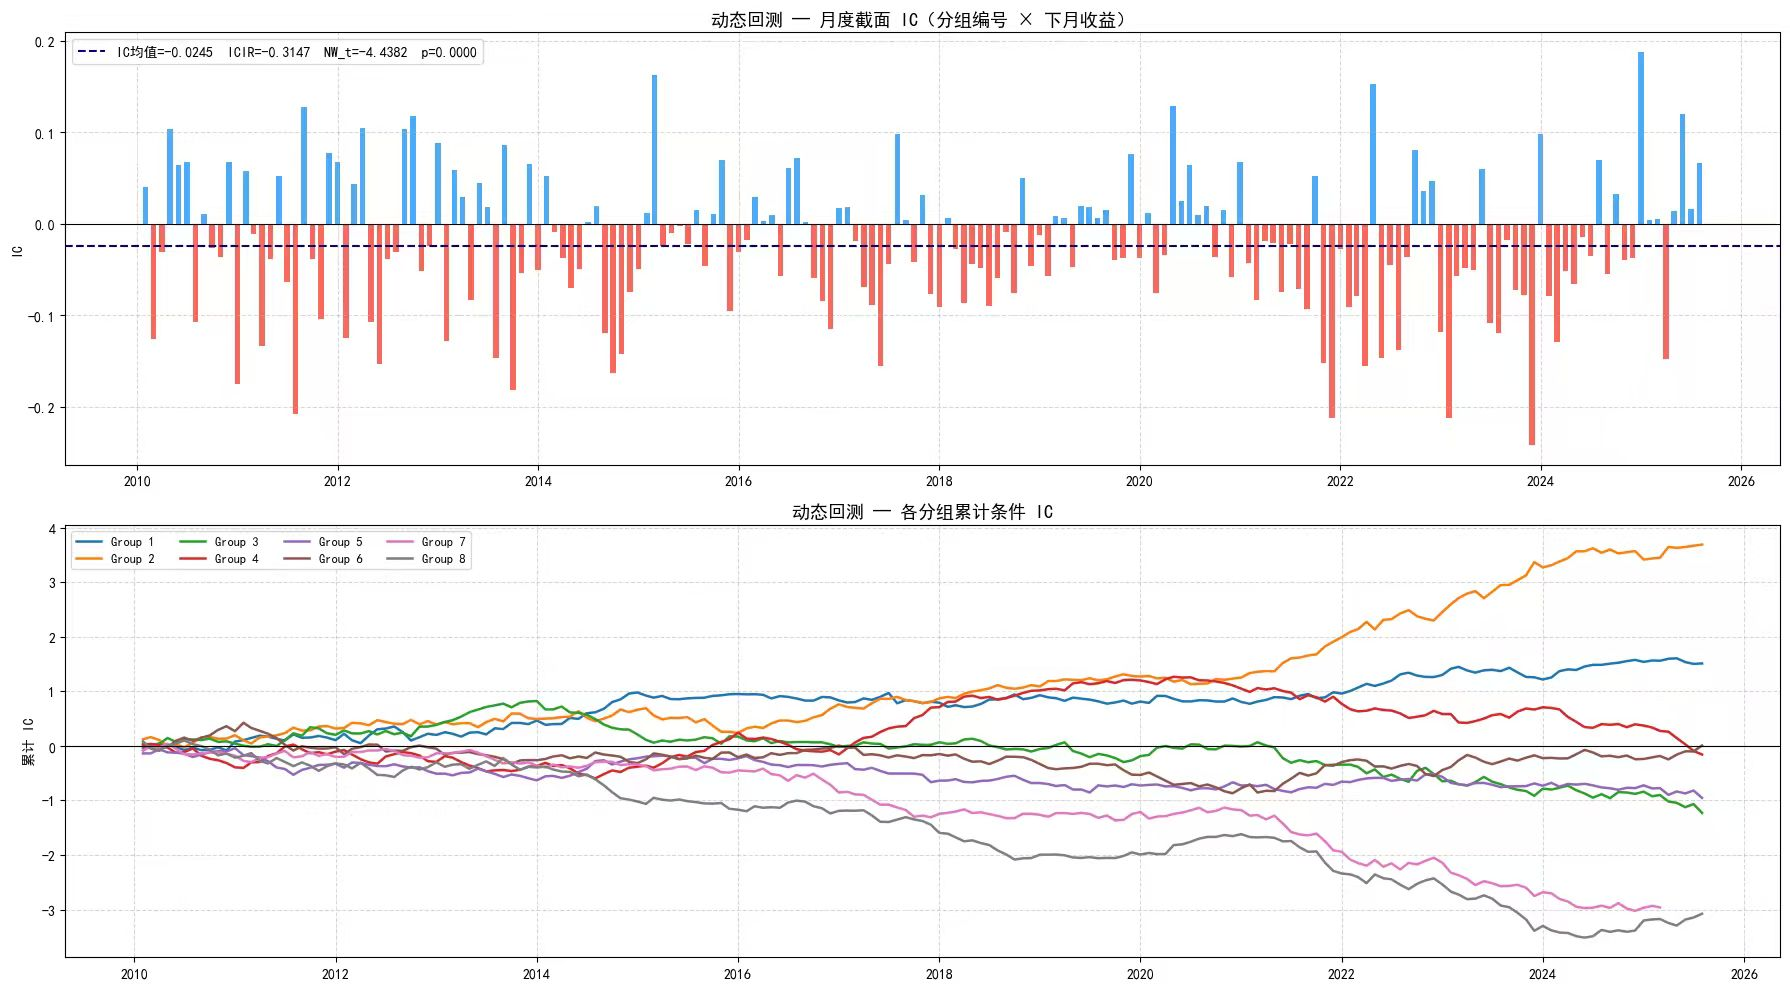
\includegraphics[width=\textwidth]{5.jpg}
    \caption{八分组动态回测净值曲线（等权与市值加权，第4格第1幅图）}
    \label{fig:8g_nav}
\end{figure}

\begin{table}[H]
\centering
\caption{八分组动态回测绩效汇总（2011--2025）}
\label{tab:8g_perf}
\begin{tabular}{@{}lrrrrrr@{}}
\toprule
\multirow{2}{*}{组别} &
\multicolumn{3}{c}{等权} &
\multicolumn{3}{c}{市值加权} \\
\cmidrule(lr){2-4}\cmidrule(lr){5-7}
 & CAGR & Sharpe & MaxDD & CAGR & Sharpe & MaxDD \\
\midrule
Group 1 & 3.25\%  & 0.254 & $-$50.5\% & 6.21\%  & 0.398 & $-$36.8\% \\
Group 2 & 5.72\%  & 0.364 & $-$40.0\% & 6.34\%  & 0.419 & $-$41.1\% \\
Group 3 & $-$2.15\% & 0.072 & $-$74.8\% & 0.05\%  & 0.133 & $-$67.4\% \\
Group 4 & 0.83\%  & 0.153 & $-$58.3\% & 6.41\%  & 0.379 & $-$63.6\% \\
Group 5 & $-$0.10\% & 0.115 & $-$60.4\% & 0.21\%  & 0.119 & $-$54.0\% \\
Group 6 & 2.24\%  & 0.210 & $-$48.5\% & 4.36\%  & 0.305 & $-$39.5\% \\
Group 7 & 0.10\%  & 0.179 & $-$78.5\% & $-$5.68\% & 0.065 & $-$91.1\% \\
Group 8 & 0.04\%  & 0.137 & $-$69.7\% & 2.96\%  & 0.241 & $-$70.4\% \\
\bottomrule
\end{tabular}
\end{table}

结果呈现几个关键规律：
\begin{enumerate}[leftmargin=2em]
    \item \textbf{FCFF 覆盖度是最强的区分变量}：Group 1--4（FCFF 充足组）整体优于 Group 5--8（FCFF 不足组），等权均值分别约为 1.9\% 和 0.6\%。
    \item \textbf{股权融资行为的负面影响}：在 FCFF 覆盖组内，有股权融资（Group 3、4）显著拖累收益；在 FCFF 不足组内，有股权融资（Group 7、8）市值加权表现尤为恶劣（Group 7 市值加权 CAGR $= -5.68\%$）。
    \item \textbf{债务融资的中性乃至正面作用}：单纯债务融资（Group 2 vs Group 1；Group 6 vs Group 5）并不拖累甚至略有提升，符合"优质企业债务融资为投资扩张服务"的预期。
\end{enumerate}

\subsubsection{截面 IC 分析}\label{subsec:ic}

\figref{5}{1} 展示了整体截面 IC 时序图及各组条件 IC 累积曲线。

\begin{figure}[H]
    \centering
    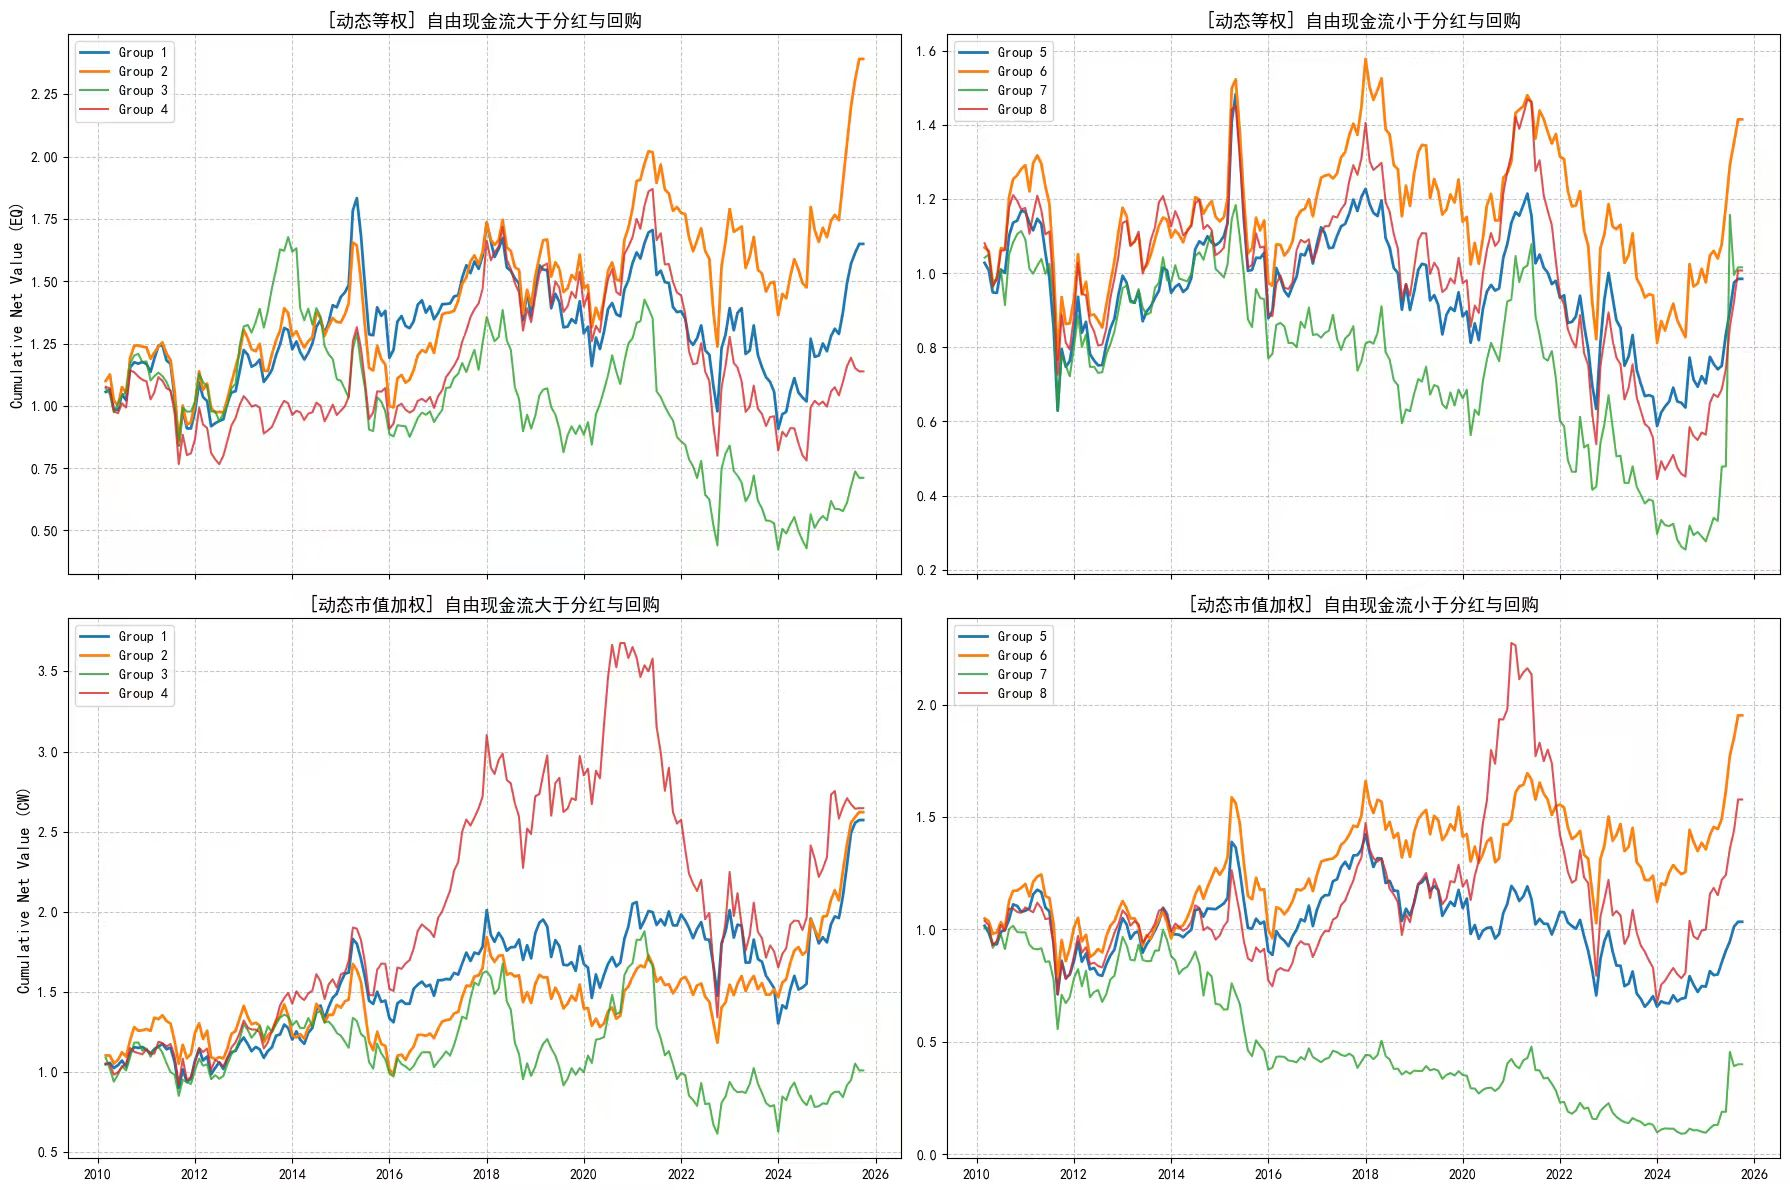
\includegraphics[width=\textwidth]{6.jpg}
    \caption{动态回测整体截面 IC（Spearman）时序与各组条件 IC（第5格第1幅图）}
    \label{fig:8g_ic}
\end{figure}

整体截面 IC 统计结果如下：

\begin{table}[H]
\centering
\caption{八分组动态回测整体截面 IC（第5格）}
\label{tab:8g_ic}
\begin{tabular}{@{}lrrrrl@{}}
\toprule
$\overline{\mathrm{IC}}$ & ICIR & NW $t$值 & $p$值 & 有效月数 & 显著性 \\
\midrule
$-0.0245$ & $-0.315$ & $-4.438$ & $<0.001$ & 187 & *** \\
\bottomrule
\end{tabular}
\end{table}

IC 为\textbf{负值}意味着：分组编号越大（Group 8），下月收益越低；
即八分组框架具有显著的\textbf{负向排序能力}——
Group 1/2 优质组的预期收益显著高于 Group 7/8 劣质组。
IC 检验采用 Newey-West HAC 标准误，不依赖净值曲线假设，
在 187 个月度观测上报告 $p < 0.001$，
排除了分组排名由多重检验或偶然噪声主导的可能。

各组条件 IC 与 BH-FDR 校正结果如下：

\begin{table}[H]
\centering
\caption{八分组各组条件 IC 与 BH-FDR 校正（第5格）}
\label{tab:8g_cond_ic}
\begin{tabular}{@{}lrrrrrr@{}}
\toprule
组别 & $\overline{\mathrm{IC}}$ & ICIR & NW $t$ & 原始$p$ & FDR $p$ & 显著性 \\
\midrule
Group 1 & $+0.0081$ & $+0.143$ & $+2.235$ & $0.025$ & $0.051$ & (边际) \\
Group 2 & $+0.0197$ & $+0.289$ & $+3.986$ & $<0.001$ & $0.001$ & *** \\
Group 3 & $-0.0066$ & $-0.100$ & $-1.380$ & $0.168$ & $0.223$ & \\
Group 4 & $-0.0008$ & $-0.013$ & $-0.141$ & $0.888$ & $0.992$ & \\
Group 5 & $-0.0051$ & $-0.102$ & $-1.498$ & $0.134$ & $0.215$ & \\
Group 6 & $+0.0000$ & $+0.001$ & $+0.010$ & $0.992$ & $0.992$ & \\
Group 7 & $-0.0163$ & $-0.260$ & $-3.542$ & $<0.001$ & $0.002$ & ** \\
Group 8 & $-0.0164$ & $-0.233$ & $-2.920$ & $0.004$ & $0.009$ & ** \\
\bottomrule
\multicolumn{7}{l}{\footnotesize BH-FDR 校正后，Group 1 的 $p=0.051$ 未通过显著性阈值（$\alpha=0.05$）。} \\
\end{tabular}
\end{table}

经 BH-FDR 校正后，Group 2（$p=0.001$）、Group 7（$p=0.002$）
和 Group 8（$p=0.009$）通过显著性检验，
而 Group 1 的 FDR 校正后 $p=0.051$，在严格意义下不显著。
这表明正向信号主要来自 Group 2（FCFF 充裕且有债务融资），
负向信号来自 Group 7/8（FCFF 不足且有股权融资）。

\subsubsection{初步结论与研究动机}

八分组结果表明：\textbf{FCFF 覆盖度}与\textbf{有无股权融资}是
影响未来截面收益最核心的两个维度，债务融资的辨别能力相对有限。
上述截面 IC 的高度显著性（$t=-4.438$，$p<0.001$）
为后续单因子验证提供了统计层面的基础支撑，
表明这一信号并非数据挖掘产物。
自然地，研究者会提出以下假说：
\begin{quote}
    \textit{若将这两个维度单独提取、连续量化，
    是否能产生单调的、统计显著的截面预测信号？}
\end{quote}

以下章节沿这一思路展开深化检验。

% =====================================================================
\subsection{动态四分组：二维分类框架的精简验证}
% =====================================================================

\subsubsection{分组逻辑}

将债务融资维度合并（不区分有无债务融资），
仅保留 FCFF 覆盖度与股权融资行为两个维度，
构成 $2 \times 2 = 4$ 个策略组：

\begin{itemize}[leftmargin=2em]
    \item \textbf{Q1}：FCFF 覆盖、无股权融资——现金流充裕、无股权稀释（最优质）
    \item \textbf{Q2}：FCFF 覆盖、有股权融资——现金流充裕，但存在股权稀释信号
    \item \textbf{Q3}：FCFF 不足、无股权融资——现金流不足，但未稀释股东
    \item \textbf{Q4}：FCFF 不足、有股权融资——现金流不足且股权稀释（最差质量）
\end{itemize}

\subsubsection{绩效结果（第8格）}

\begin{table}[H]
\centering
\caption{动态四分组回测绩效（2011--2025，第8格）}
\label{tab:4g_perf}
\begin{tabular}{@{}lrrrrrrl@{}}
\toprule
\multirow{2}{*}{组别} &
\multicolumn{3}{c}{等权} &
\multicolumn{3}{c}{市值加权} &
\multirow{2}{*}{月均N} \\
\cmidrule(lr){2-4}\cmidrule(lr){5-7}
 & CAGR & Sharpe & MaxDD & CAGR & Sharpe & MaxDD & \\
\midrule
Q1（FCFF 覆盖，无融资） & 5.08\%  & 0.338 & $-$40.1\% & 6.45\%  & 0.433 & $-$37.0\% & 142.8 \\
Q2（FCFF 覆盖，有融资） & 1.09\%  & 0.164 & $-$60.2\% & 5.40\%  & 0.340 & $-$64.6\% & 70.0 \\
Q3（FCFF 不足，无融资） & 1.75\%  & 0.190 & $-$50.0\% & 3.54\%  & 0.269 & $-$40.9\% & 121.8 \\
Q4（FCFF 不足，有融资） & $-$0.18\% & 0.130 & $-$70.6\% & 1.22\%  & 0.177 & $-$71.1\% & 87.3 \\
\bottomrule
\end{tabular}
\end{table}

四分组框架呈现出差序分明的排列，但并非严格单调：
等权 CAGR 实际顺序为 Q1（5.08\%）$>$ Q3（1.75\%）$>$ Q2（1.09\%）$>$ Q4（$-$0.18\%）。
值得注意的是，\textbf{Q2（FCFF 充裕但有股权融资）的表现低于 Q3（FCFF 不足但无股权融资）}，
说明股权融资行为的负面效应甚至超过了 FCFF 覆盖不足本身——
即对于二元分类而言，\textbf{股权稀释}比现金流质量偏弱更具决定性的负面作用。
这一发现与八分组框架高度一致：有股权融资的 Group 3/4 整体劣于无外部融资的 Group 5。

\subsubsection{截面 IC 分析（第9格）}

\begin{table}[H]
\centering
\caption{动态四分组整体及各组条件 IC（第9格，BH-FDR 校正）}
\label{tab:4g_ic}
\begin{tabular}{@{}lrrrrrr@{}}
\toprule
层面 & $\overline{\mathrm{IC}}$ & ICIR & NW $t$ & 原始$p$ & FDR $p$ & 显著性 \\
\midrule
整体 IC & $+0.0268$ & $+0.337$ & $+4.709$ & $<0.001$ & $<0.001$ & *** \\
Q1（FCFF 覆盖，无融资） & $+0.0233$ & $+0.317$ & $+4.483$ & $<0.001$ & $<0.001$ & *** \\
Q2（FCFF 覆盖，有融资） & $-0.0031$ & $-0.044$ & $-0.487$ & $0.626$ & $0.626$ & \\
Q3（FCFF 不足，无融资） & $-0.0027$ & $-0.041$ & $-0.555$ & $0.579$ & $0.626$ & \\
Q4（FCFF 不足，有融资） & $-0.0225$ & $-0.289$ & $-3.504$ & $<0.001$ & $0.001$ & *** \\
\bottomrule
\multicolumn{7}{l}{\footnotesize IC$>$0 占比 64.7\%；整体 IC 中位数 $= 0.066$。} \\
\end{tabular}
\end{table}

整体 IC 为正值且高度显著（$t=+4.709$，$p<0.001$，187 个月），
表明 Q\_score 越高（Q1 最高，Q4 最低），下月收益越高。
BH-FDR 校正后，Q1 和 Q4 均通过显著性检验——
Q1 作为"质量最高"组的成员身份与高收益显著正相关（$p<0.001$），
Q4 作为"质量最低"组的成员身份与低收益显著负相关（$p<0.001$）。
Q2 和 Q3 的条件 IC 不显著，说明在固定一个维度后，
另一维度的区分力依赖于两者的联合出现。

上述结果与第~\ref{subsec:ic}节中八分组整体 IC（$p<0.001$）高度呼应，
进一步确认了 FCFF 覆盖度与股权融资行为二维分类框架的有效性，
同时证明在合并债务融资维度后信号强度并未衰减（ICIR 从 0.315 提升至 0.337）。

% =====================================================================
\subsection{深化检验：双重排序的局限性}
% =====================================================================

\subsubsection{5 $\times$ 5 双重排序（第11格）}

将 FCFF 覆盖率强度（F1 弱至 F5 强）与股权融资强度（E1 零融资至 E5 高融资）
分别五等分，构成 25 个交叉组合（第11格）。
\figref{11}{1} 展示了各单元格等权 CAGR 热力图。

\begin{figure}[H]
    \centering
    
\includegraphics[width=0.85\textwidth]{4.png}
    \caption{5$\times$5 双重排序等权 CAGR 热力图（第11格第1幅图）}
    \label{fig:25g_heatmap}
\end{figure}

\begin{table}[H]
\centering
\caption{5$\times$5 双重排序等权 CAGR（2011--2025，第11格）}
\label{tab:25g_cagr}
\begin{tabular}{@{}lccccc@{}}
\toprule
 & E1(零融资) & E2(融资Q1) & E3(融资Q2) & E4(融资Q3) & E5(融资Q4) \\
\midrule
F1(覆盖↓) & $-2.64\%$ & $13.18\%$ & $-6.34\%$ & $-25.01\%$ & $-17.87\%$ \\
F2        & $6.63\%$  & $3.52\%$  & $6.95\%$  & $-16.67\%$ & $-3.20\%$ \\
F3        & $1.34\%$  & $7.12\%$  & $-12.35\%$& $-1.27\%$  & $24.34\%$ \\
F4        & $1.45\%$  & $-16.86\%$& $-4.40\%$ & $-7.09\%$  & $-18.68\%$ \\
F5(覆盖↑) & $2.96\%$  & $-2.90\%$ & $-1.21\%$ & $21.56\%$  & $-2.91\%$ \\
\bottomrule
\end{tabular}
\end{table}

表~\ref{tab:25g_cagr} 呈现出明显的\textbf{非单调性}和\textbf{噪声主导}的特征：
单元格（F3, E5）的 CAGR 高达 24.34\%，而邻近单元格（F1, E4）为 $-25.01\%$，
这种极端跳跃难以用经济逻辑解释。

原因在于\textbf{样本量极度不足}：
第12格数据显示，E2--E5 各列的月均持股数量仅为 0.7--1.6 只（见表~\ref{tab:12g_n}），
绝大多数单元格每月仅持有不足 2 只股票。

\begin{table}[H]
\centering
\caption{5$\times$5 双重排序各组月均持股数量（第12格）}
\label{tab:12g_n}
\begin{tabular}{@{}lccccc@{}}
\toprule
 & E1(零融资) & E2(融资Q1) & E3(融资Q2) & E4(融资Q3) & E5(融资Q4) \\
\midrule
F1(覆盖↓) & 9.5 & 1.3 & 1.1 & 1.3 & 1.6 \\
F2        & 9.5 & 1.2 & 1.2 & 1.3 & 0.9 \\
F3        & 9.6 & 1.1 & 1.4 & 1.1 & 0.9 \\
F4        & 9.3 & 1.5 & 1.1 & 1.0 & 1.2 \\
F5(覆盖↑) & 10.9 & 0.9 & 0.8 & 0.7 & 1.2 \\
\bottomrule
\multicolumn{6}{l}{\footnotesize 注：E2--E5 各列月均持股数均低于 2 只，不具备统计检验能力。} \\
\end{tabular}
\end{table}

在如此稀疏的截面下，任何绩效数字均被个股特质风险所主导，毫无统计意义。

\subsubsection{5 $\times$ 2 双重排序（第13/14格）}

将股权融资维度压缩为二元分类（E0: 无股权融资，E1: 有股权融资），
与 FCFF 覆盖率五等分构成 10 个组合（第13格）。

\begin{table}[H]
\centering
\caption{5$\times$2 双重排序各组月均持股数量及 CAGR（第13格）}
\label{tab:10g_summary}
\begin{tabular}{@{}lrrrr@{}}
\toprule
组别 & 月均N(E0) & 月均N(E1) & EQ CAGR(E0) & EQ CAGR(E1) \\
\midrule
F1(覆盖↓) & 9.5 & 5.3 & $-$2.64\% & $-$0.25\% \\
F2        & 9.5 & 4.9 & 6.63\%    & 5.19\% \\
F3        & 9.8 & 4.9 & 1.34\%    & 5.49\% \\
F4        & 10.0 & 4.9 & 1.45\%   & 0.50\% \\
F5(覆盖↑) & 11.0 & 3.9 & 2.96\%  & $-$0.01\% \\
\bottomrule
\multicolumn{5}{l}{\footnotesize E0（无融资）月均合计约 50 只；E1（有融资）月均合计约 24 只。} \\
\end{tabular}
\end{table}

F 轴 IC 在两个子集内分别计算如下（第14格）：

\begin{table}[H]
\centering
\caption{5$\times$2 双重排序 F 轴截面 IC（第14格）}
\label{tab:10g_ic}
\begin{tabular}{@{}lrrrl@{}}
\toprule
子集 & $\overline{\mathrm{IC}}$ & ICIR & NW $p$值 & 显著性 \\
\midrule
E0（零融资） & $+0.0077$ & 0.038 & 0.658 & n.s. \\
E1（有融资） & $+0.0030$ & 0.011 & 0.864 & n.s. \\
整体（E0+E1）& $+0.0102$ & 0.067 & 0.345 & n.s. \\
\bottomrule
\end{tabular}
\end{table}

多空组合（Long F5E0 / Short F1E1）等权与市值加权均不显著
（$p = 0.997$ 与 $p = 0.815$）。
所有 10 组在 BH-FDR 校正后 $p$ 值均超过 0.48（表~\ref{tab:10g_nw}）。

\begin{table}[H]
\centering
\caption{5$\times$2 双重排序各组 NW $t$ 检验（第14格，BH-FDR 校正）}
\label{tab:10g_nw}
\begin{tabular}{@{}lrrrrrr@{}}
\toprule
组别 & 月均(EQ) & $t$(EQ) & $p$(EQ) & FDR $p$(EQ) & $p$(CW) & FDR $p$(CW) \\
\midrule
F1E0 & $0.095\%$ & 0.157 & 0.875 & 0.875 & 0.779 & 0.866 \\
F1E1 & $0.497\%$ & 0.724 & 0.469 & 0.521 & 0.410 & 0.556 \\
F2E0 & $0.891\%$ & 1.496 & 0.135 & 0.521 & 0.099 & 0.484 \\
F2E1 & $0.872\%$ & 1.277 & 0.202 & 0.521 & 0.194 & 0.484 \\
F3E0 & $0.503\%$ & 0.813 & 0.416 & 0.521 & 0.936 & 0.936 \\
F3E1 & $0.828\%$ & 1.406 & 0.160 & 0.521 & 0.150 & 0.484 \\
F4E0 & $0.449\%$ & 0.829 & 0.407 & 0.521 & 0.445 & 0.556 \\
F4E1 & $0.559\%$ & 0.754 & 0.451 & 0.521 & 0.053 & 0.484 \\
F5E0 & $0.490\%$ & 1.058 & 0.290 & 0.521 & 0.423 & 0.556 \\
F5E1 & $0.473\%$ & 0.799 & 0.424 & 0.521 & 0.357 & 0.556 \\
\bottomrule
\end{tabular}
\end{table}

此外，沿 F 轴折叠后各行 CAGR（$-1.44\%,\;5.91\%,\;3.42\%,\;0.98\%,\;1.48\%$）
呈明显非单调形态，进一步证明连续型覆盖率信号在此样本中无法提取。
沿 E 轴折叠则显示 E0（无融资）与 E1（有融资）的等权 CAGR 几乎无差异（$1.95\%$ vs $2.19\%$），
表明股权融资维度在此截面规模下的独立解释力接近于零。

\textbf{关键结论}：
双重排序框架在本样本规模下因截面样本不足而失去检验能力。
然而，这\textbf{不能}等同于"FCFF 覆盖率维度无效"——
对比第~\ref{subsec:ic}节中八分组整体 IC（$p<0.001$，全样本月均参与股票逾 200 只），
这一检验能力的崩塌印证：样本碎片化是双重排序失效的根本原因，而非底层信号的消失。

此外，亦存在一种值得记录的经济视角：
若市场中 FCFF 充裕度极高且同时大量进行股权融资的企业天然稀少，
这或许反映两个维度在现实公司财务决策中的内在相关性——
现金流高度充裕的企业一般较少有补充股权资本的迫切需求。
当前数据无法区分"样本量不足"与"经济互斥"这两种解释，两者均值得记录。

% =====================================================================
\subsection{CFO 类因子：覆盖率与收益率的多维检验}
% =====================================================================

双重排序的失效源于连续化处理导致的样本碎片化，而非底层维度无效。
由此，研究策略转向\textbf{单因子框架}：
放弃对 FCFF 覆盖度与股权融资行为的同时连续量化，
转而在\textbf{单一维度}上集中提取信号。
CFO 覆盖率可视为八分组框架中 FCFF 覆盖度维度的连续量化版本——
在全体有分配行为的企业截面上对该维度的强度进行排序，
既保留了八分组框架中最有效的区分轴，又避免了双重排序引入的截面碎片化问题。

\subsubsection{CFO 覆盖率单因子（第16格）}

鉴于双重排序在样本量层面的根本局限，
研究转向单因子框架，
在全有效样本（有分配行为的企业，月均 283 只）上
对连续型 FCFF 代理因子——
CFO 覆盖率（$\mathrm{CFO\,Coverage} = \mathrm{CFO} / (\mathrm{Div} + \mathrm{Buyback})$）——
进行五等分排序。

\begin{figure}[H]
    \centering
    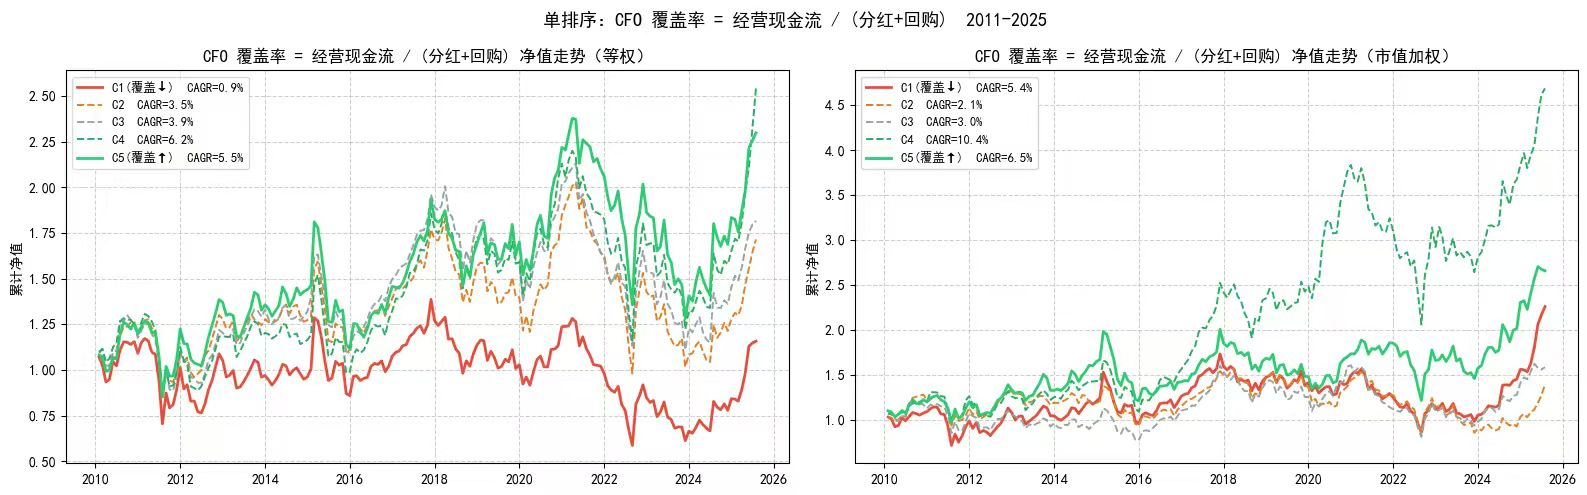
\includegraphics[width=\textwidth]{3.jpg}
    \caption{CFO 覆盖率五等分净值曲线（第16格第1幅图）}
    \label{fig:cfo_nav}
\end{figure}

\begin{table}[H]
\centering
\caption{CFO 覆盖率单因子回测绩效（第16格，样本：有分配企业，月均 283 只）}
\label{tab:cfo_perf}
\begin{tabular}{@{}lrrrrrrl@{}}
\toprule
组别 & EQ CAGR & EQ Sharpe & EQ MaxDD & CW CAGR & CW Sharpe & CW MaxDD & 月均N \\
\midrule
C1（覆盖↓） & $0.94\%$  & 0.161 & $-57.7\%$ & $5.36\%$  & 0.344 & $-50.4\%$ & 57.0 \\
C2          & $3.52\%$  & 0.264 & $-51.7\%$ & $2.13\%$  & 0.204 & $-46.1\%$ & 56.5 \\
C3          & $3.90\%$  & 0.283 & $-47.9\%$ & $2.99\%$  & 0.245 & $-49.6\%$ & 56.4 \\
C4          & $6.17\%$  & 0.369 & $-47.3\%$ & $10.42\%$ & 0.572 & $-46.3\%$ & 56.5 \\
C5（覆盖↑） & $5.48\%$  & 0.339 & $-46.1\%$ & $6.47\%$  & 0.402 & $-39.6\%$ & 56.8 \\
\midrule
\multicolumn{2}{@{}l}{多空（C5$-$C1）等权} & \multicolumn{2}{l}{CAGR $= 3.81\%$} &
\multicolumn{2}{l}{$t = +2.398$} & \multicolumn{2}{l}{$p = 0.017$\,*} \\
\multicolumn{2}{@{}l}{多空（C5$-$C1）市值加权} & \multicolumn{2}{l}{CAGR $= 0.22\%$} &
\multicolumn{2}{l}{$t = +0.261$} & \multicolumn{2}{l}{$p = 0.794$\,n.s.} \\
\bottomrule
\end{tabular}
\end{table}

等权 CAGR 从 C1 至 C4 呈递增趋势（0.94\%、3.52\%、3.90\%、6.17\%），
但\textbf{C5（5.48\%）低于 C4（6.17\%）}，非严格单调。
等权多空 CAGR 达 3.81\%，NW $t$ 检验在 5\% 水平显著（$p=0.017$）；
但市值加权多空完全不显著（$p=0.794$），
说明该信号主要集中于等权意义下的小市值股票，市值加权后不稳定。

截面 IC 检验结果如下：

\begin{table}[H]
\centering
\caption{CFO 覆盖率截面 IC 与 NW $t$ 检验（第16格）}
\label{tab:cfo_ic}
\begin{tabular}{@{}lrrrrl@{}}
\toprule
层面 & $\overline{\mathrm{IC}}$ & ICIR & NW $t$ & $p$值 & 显著性 \\
\midrule
截面 IC（Spearman） & $+0.0120$ & $+0.188$ & $+2.862$ & $0.004$ & ** \\
\bottomrule
\end{tabular}
\end{table}

截面 IC 在 1\% 水平显著（$p=0.004$），
IC 的统计显著性独立于净值曲线的单调性观察，
排除了 C1--C5 收益梯度由偶然噪声主导的假设。

\figref{16}{2} 展示了 IC 时序与累积 IC 图。

\begin{figure}[H]
    \centering
    
\includegraphics[width=\textwidth]{2.png}
    \caption{CFO 覆盖率截面 IC 时序与累积 IC（第16格第2幅图）}
    \label{fig:cfo_ic}
\end{figure}

\subsubsection{CFO 覆盖率严格筛选版（第19格）}\label{subsec:cfo_strict}

进一步对 CFO 覆盖率因子施加月度 p25 分配强度过滤，
结果信号\textbf{完全消失}：

\begin{table}[H]
\centering
\caption{CFO 覆盖率严格筛选版 IC 对比（第19格）}
\label{tab:cfo_strict}
\begin{tabular}{@{}llrrrl@{}}
\toprule
版本 & 月均样本量 & $\overline{\mathrm{IC}}$ & ICIR & NW $p$值 & 显著性 \\
\midrule
原版（全有分配样本） & 283 只 & $+0.0120$ & $+0.188$ & $0.004$ & ** \\
严格版（剔除 p25）   & 54 只  & $+0.0005$ & $+0.003$ & $0.970$ & n.s. \\
\bottomrule
\end{tabular}
\end{table}

样本量从 283 只减少至 54 只后信号完全消失。
这一结果至少有两种解读，两者目前无法区分：
\begin{itemize}[leftmargin=2em]
    \item \textbf{截面规模解释}：因子信号对样本量高度敏感，54 只的截面不具备统计功效；
    \item \textbf{分母趋零解释}：原版信号部分或全部由绝对分配金额极小（$\mathrm{Div}+\mathrm{Buyback} \to 0$）的企业驱动——这类企业的 CFO Coverage 因分母趋零而呈现极大值，被机械地排入 C5 高分位，但其高"覆盖率"并不反映真实的经营现金流充裕，仅是除法运算的数学伪影。剔除此类企业后信号消失，与该假说高度相符。
\end{itemize}
在无法区分两种解释的情况下，对 CFO Coverage IC 显著性的解读应保持保守。

\subsubsection{CFO Yield（第21格）}

CFO Yield 直接将 CFO 对市值取比率（$\mathrm{CFO\,Yield} = \mathrm{CFO} / \mathrm{Market\,Cap}$），
以全样本（有 CFO 数据的企业，月均 110 只）进行五等分排序。
注意 CFO Coverage $\times$ (Div+Buyback)/MktCap $=$ CFO Yield，
两者衡量维度不同（前者为对股东回报的覆盖倍数，后者为 CFO 收益率）。

\begin{table}[H]
\centering
\caption{CFO Yield 单因子回测绩效（第21格，月均 110 只）}
\label{tab:cfy_perf}
\begin{tabular}{@{}lrrrrrrl@{}}
\toprule
组别 & EQ CAGR & EQ Sharpe & EQ MaxDD & CW CAGR & CW Sharpe & CW MaxDD & 月均N \\
\midrule
CY1（低） & $-5.08\%$ & $-$0.050 & $-91.0\%$ & $3.61\%$ & 0.266 & $-65.9\%$ & 22.4 \\
CY2       & $2.13\%$ & 0.207 & $-69.3\%$ & $4.47\%$ & 0.302 & $-53.9\%$ & 21.8 \\
CY3       & $5.97\%$ & 0.360 & $-39.5\%$ & $1.18\%$ & 0.164 & $-58.1\%$ & 21.7 \\
CY4       & $4.70\%$ & 0.308 & $-54.9\%$ & $0.70\%$ & 0.156 & $-60.7\%$ & 21.8 \\
CY5（高） & $4.51\%$ & 0.296 & $-44.5\%$ & $5.74\%$ & 0.362 & $-41.7\%$ & 22.1 \\
\midrule
\multicolumn{2}{@{}l}{多空（CY5$-$CY1）等权} & \multicolumn{2}{l}{CAGR $= 8.61\%$} &
\multicolumn{2}{l}{$t = +2.445$} & \multicolumn{2}{l}{$p = 0.015$\,*} \\
\multicolumn{2}{@{}l}{多空（CY5$-$CY1）市值加权} & \multicolumn{2}{l}{CAGR $= 0.54\%$} &
\multicolumn{2}{l}{$t = +0.415$} & \multicolumn{2}{l}{$p = 0.678$\,n.s.} \\
\bottomrule
\end{tabular}
\end{table}

等权 CAGR 呈高度不对称形态：CY1 极低（$-5.08\%$），远低于其余各组；
CY2--CY5 均为正值（$2.13\%$、$5.97\%$、$4.70\%$、$4.51\%$），
其中 CY3（$5.97\%$）为全组最高点，CY4/CY5 小幅回落，形成右侧截断的不对称结构，非严格单调。
截面 IC：

\begin{table}[H]
\centering
\caption{CFO Yield 截面 IC（第21格）}
\label{tab:cfy_ic}
\begin{tabular}{@{}lrrrrl@{}}
\toprule
$\overline{\mathrm{IC}}$ & ICIR & NW $t$ & $p$值 & 显著性 \\
\midrule
$+0.0320$ & $+0.222$ & $+2.941$ & $0.003$ & ** \\
\bottomrule
\end{tabular}
\end{table}

截面 IC 在 1\% 水平显著（$p=0.003$），等权多空亦显著（$p=0.015$），
市值加权多空不显著（$p=0.678$）。
信号模式与 CFO Coverage 类似：等权有效，市值加权消失，
同样受限于月均仅 110 只的截面规模。

\subsubsection{TTM 滚动 CFO Yield（第22格）}

TTM CFO Yield 利用半年报数据构建滚动十二月经营现金流：
\[
    \mathrm{TTM\_CFO}(t) = \mathrm{CFO\_Annual}(t) + \mathrm{CFO\_H1}(t+1) - \mathrm{CFO\_H1}(t)
\]
将信号刷新频率从年度提升至半年度，样本覆盖月均 159 只股票。

\begin{table}[H]
\centering
\caption{TTM CFO Yield 单因子回测绩效（第22格，月均 159 只）}
\label{tab:ttm_perf}
\begin{tabular}{@{}lrrrrrrl@{}}
\toprule
组别 & EQ CAGR & EQ Sharpe & EQ MaxDD & CW CAGR & CW Sharpe & CW MaxDD & 月均N \\
\midrule
T1（低） & $-4.42\%$ & $-$0.023 & $-85.6\%$ & $6.27\%$ & 0.372 & $-41.0\%$ & 32.2 \\
T2       & $-0.16\%$ & 0.112  & $-74.4\%$ & $5.69\%$ & 0.359 & $-48.9\%$ & 31.5 \\
T3       & $3.36\%$  & 0.255  & $-56.6\%$ & $0.14\%$ & 0.109 & $-62.1\%$ & 31.6 \\
T4       & $5.28\%$  & 0.333  & $-43.2\%$ & $6.07\%$ & 0.360 & $-42.9\%$ & 31.5 \\
T5（高） & $4.04\%$  & 0.277  & $-44.3\%$ & $4.83\%$ & 0.323 & $-38.6\%$ & 32.0 \\
\midrule
\multicolumn{2}{@{}l}{多空（T5$-$T1）等权} & \multicolumn{2}{l}{CAGR $= 7.46\%$} &
\multicolumn{2}{l}{$t = +2.446$} & \multicolumn{2}{l}{$p = 0.015$\,*} \\
\multicolumn{2}{@{}l}{多空（T5$-$T1）市值加权} & \multicolumn{2}{l}{CAGR $= -2.52\%$} &
\multicolumn{2}{l}{$t = -0.582$} & \multicolumn{2}{l}{$p = 0.561$\,n.s.} \\
\bottomrule
\end{tabular}
\end{table}

等权 CAGR 从 T1 至 T4 递增，但 T5（4.04\%）低于 T4（5.28\%），
与 CFO Coverage 和 CFO Yield 呈现相同的"C4/T4 顶部"非单调形态。
截面 IC 为本研究中 CFO 类因子的最高水平：

\begin{table}[H]
\centering
\caption{TTM CFO Yield 截面 IC（第22格）}
\label{tab:ttm_ic}
\begin{tabular}{@{}lrrrrl@{}}
\toprule
$\overline{\mathrm{IC}}$ & ICIR & NW $t$ & $p$值 & 显著性 \\
\midrule
$+0.0272$ & $+0.248$ & $+3.164$ & $0.002$ & ** \\
\bottomrule
\end{tabular}
\end{table}

截面 IC 在 1\% 水平显著（$p=0.002$），等权多空亦显著（$p=0.015$），
市值加权不显著（$p=0.561$）。
TTM 信号通过提升刷新频率增加了月度观测的有效性（月均 159 只 vs 110 只），
可能是该组因子中信号最稳健的版本。

% =====================================================================
\subsection{净股东回报收益率（NPY）：两个截面版本的比较}
% =====================================================================

\subsubsection{NPY 的构建逻辑}

净股东回报收益率（Net Payout Yield，NPY）将分配能力与股权融资行为合并为单一信号：
\[
    \mathrm{NPY} = \frac{\mathrm{Div} + \mathrm{Buyback} - \mathrm{Equity\_Issuance}}{\mathrm{Market\,Cap}}
\]
其经济含义为：企业每单位市值净流回股东的现金。
NPY 高意味着公司慷慨分配且克制股权融资，在方向上与 Q1/Q2 特征一致。
然而，NPY 的分母为市值，衡量的是净回报\textbf{收益率}，
而非 FCFF 对分配的\textbf{覆盖倍数}——
即使是 Group 1 公司，若市值较大而分配绝对额偏小，其 NPY 也可能偏低。
这一结构差异决定了 NPY 与 FCFF 覆盖度信号在本质上测量不同维度。

\subsubsection{NPY 全样本版（第15格）}

以全部有 NPY 数据的企业（含 NPY $\leq 0$ 的净融资企业）作为截面，
月均 110 只股票（原始 NPY 计算基础 12,233 行，2,836 只股票；
其中 NPY $> 0$ 者 4,171 条记录，NPY $\leq 0$ 者 8,062 条记录）：

\begin{table}[H]
\centering
\caption{NPY 全样本版回测绩效（第15格，月均 110 只）}
\label{tab:npy_full_perf}
\begin{tabular}{@{}lrrrrrrl@{}}
\toprule
组别 & EQ CAGR & EQ Sharpe & EQ MaxDD & CW CAGR & CW Sharpe & CW MaxDD & 月均N \\
\midrule
N1（融资↑） & $-2.26\%$ & 0.049 & $-82.7\%$ & $3.43\%$ & 0.260 & $-65.7\%$ & 22.4 \\
N2          & $1.85\%$  & 0.196 & $-64.4\%$ & $1.41\%$ & 0.175 & $-59.3\%$ & 21.8 \\
N3          & $3.09\%$  & 0.247 & $-68.9\%$ & $2.97\%$ & 0.242 & $-51.7\%$ & 21.7 \\
N4          & $5.12\%$  & 0.326 & $-51.1\%$ & $4.03\%$ & 0.282 & $-52.1\%$ & 21.8 \\
N5（回报↑） & $3.99\%$  & 0.274 & $-55.0\%$ & $7.98\%$ & 0.448 & $-42.2\%$ & 22.1 \\
\midrule
\multicolumn{2}{@{}l}{多空（N5$-$N1）等权} & \multicolumn{2}{l}{CAGR $= 5.10\%$} &
\multicolumn{2}{l}{$t = +1.587$} & \multicolumn{2}{l}{$p = 0.113$\,n.s.} \\
\multicolumn{2}{@{}l}{多空（N5$-$N1）市值加权} & \multicolumn{2}{l}{CAGR $= 1.45\%$} &
\multicolumn{2}{l}{$t = +0.729$} & \multicolumn{2}{l}{$p = 0.466$\,n.s.} \\
\bottomrule
\end{tabular}
\end{table}

等权 CAGR 从 N1 至 N4 递增，但 N5（3.99\%）低于 N4（5.12\%），
再次呈现本研究中普遍出现的"第四分位顶部"非单调形态。
截面 IC：

\begin{table}[H]
\centering
\caption{NPY 全样本版截面 IC（第15格）}
\label{tab:npy_full_ic}
\begin{tabular}{@{}lrrrrl@{}}
\toprule
$\overline{\mathrm{IC}}$ & ICIR & NW $t$ & $p$值 & 显著性 \\
\midrule
$+0.0246$ & $+0.177$ & $+2.367$ & $0.018$ & * \\
\bottomrule
\end{tabular}
\end{table}

截面 IC 在 5\% 水平边际显著（$p=0.018$），
但多空组合等权（$p=0.113$）和市值加权（$p=0.466$）均不显著。
BH-FDR 校正后各组均未通过显著性阈值。

\subsubsection{NPY 有分配子集版（第18格）}

进一步将截面限定于有实际分配行为（$\mathrm{Div}+\mathrm{Buyback} > 0$）的企业，
月均 72 只，原始样本 4,615 行，1,592 只股票：

\begin{figure}[H]
    \centering
    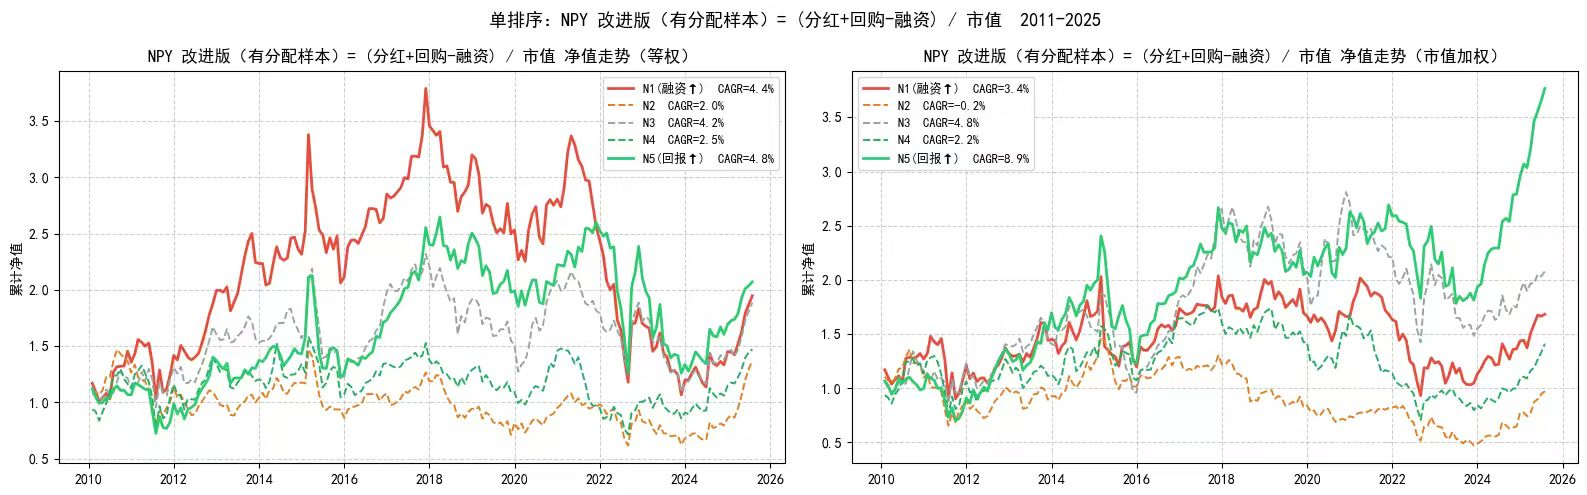
\includegraphics[width=\textwidth]{1.jpg}
    \caption{NPY 有分配版五等分净值曲线（第18格第1幅图）}
    \label{fig:npy_nav}
\end{figure}

\begin{table}[H]
\centering
\caption{NPY 有分配版回测绩效（第18格，月均 72 只）}
\label{tab:npy_perf}
\begin{tabular}{@{}lrrrrrrl@{}}
\toprule
组别 & EQ CAGR & EQ Sharpe & EQ MaxDD & CW CAGR & CW Sharpe & CW MaxDD & 月均N \\
\midrule
N1（融资↑） & $4.37\%$ & 0.285 & $-71.9\%$ & $3.40\%$ & 0.261 & $-54.3\%$ & 14.7 \\
N2          & $2.04\%$ & 0.203 & $-58.0\%$ & $-0.18\%$& 0.114 & $-67.9\%$ & 14.1 \\
N3          & $4.16\%$ & 0.286 & $-52.9\%$ & $4.80\%$ & 0.309 & $-49.3\%$ & 14.1 \\
N4          & $2.51\%$ & 0.223 & $-54.8\%$ & $2.24\%$ & 0.212 & $-59.9\%$ & 14.1 \\
N5（回报↑） & $4.78\%$ & 0.295 & $-52.6\%$ & $8.88\%$ & 0.468 & $-48.9\%$ & 14.5 \\
\midrule
\multicolumn{2}{@{}l}{多空（N5$-$N1）等权} & \multicolumn{2}{l}{CAGR $= -0.80\%$} &
\multicolumn{2}{l}{$t = +0.170$} & \multicolumn{2}{l}{$p = 0.865$\,n.s.} \\
\multicolumn{2}{@{}l}{多空（N5$-$N1）市值加权} & \multicolumn{2}{l}{CAGR $= 2.76\%$} &
\multicolumn{2}{l}{$t = +1.107$} & \multicolumn{2}{l}{$p = 0.268$\,n.s.} \\
\bottomrule
\end{tabular}
\end{table}

\begin{table}[H]
\centering
\caption{NPY 有分配版截面 IC（第18格）}
\label{tab:npy_ic}
\begin{tabular}{@{}lrrrrl@{}}
\toprule
$\overline{\mathrm{IC}}$ & ICIR & NW $t$ & $p$值 & 显著性 \\
\midrule
$-0.0014$ & $-0.008$ & $-0.114$ & $0.909$ & n.s. \\
\bottomrule
\end{tabular}
\end{table}

在有分配子集上，NPY 的截面 IC 接近零（$\overline{\mathrm{IC}} = -0.001$），
$p=0.909$，信号完全消失。
等权 CAGR 呈完全无规律的振荡（4.37\%、2.04\%、4.16\%、2.51\%、4.78\%），
无单调性可言。

\subsubsection{两个版本的对比解读}

\begin{table}[H]
\centering
\caption{NPY 两版本 IC 对比}
\label{tab:npy_compare}
\begin{tabular}{@{}lrrrrl@{}}
\toprule
版本 & 截面定义 & 月均N & $\overline{\mathrm{IC}}$ & NW $p$ & 显著性 \\
\midrule
全样本版（第15格） & 全部有NPY数据 & 110 & $+0.0246$ & $0.018$ & * \\
有分配版（第18格） & 仅有分配行为 & 72  & $-0.0014$ & $0.909$ & n.s. \\
\bottomrule
\end{tabular}
\end{table}

两个版本截面定义不同，结论迥异。
全样本版包含 NPY $\leq 0$ 的净融资企业，
这些企业（股权融资额超过分配额）往往绩效较差，
导致 N1 组等权 CAGR 低至 $-2.26\%$，由此人为放大了 N1 至 N5 的收益差距。
有分配版剔除了净融资企业，截面仅剩纯粹的"分配强度排名"，
信号随即消失。
这说明 NPY 的全样本 IC 信号主要来源于\textbf{是否净融资}这一二元维度，
而非 NPY 数值高低的连续排序能力——这与第四节动态四分组中
Q4 条件 IC 显著负向（$p<0.001$，见表~\ref{tab:4g_ic}）的结论形成呼应：
股权融资行为的负面效应在二元分类框架下是真实且显著的，
但经 NPY 连续化并引入市值分母后，信号被稀释至消失。

% =====================================================================
\subsection{讨论}
% =====================================================================

\subsubsection{对研究发现的综合解读}

本研究沿三条主线推进：（1）二元分类框架（八分组、四分组）；
（2）连续因子双重排序；（3）单因子检验。
各条主线的统计结论高度自洽：

\begin{enumerate}[leftmargin=2em]
    \item \textbf{二元分类有效}：无论是八分组（IC $p<0.001$）
    还是动态四分组（IC $p<0.001$），
    FCFF 覆盖度与股权融资行为的联合二元分类均给出了
    统计显著的截面排序能力，且 BH-FDR 校正后仍然成立。

    \item \textbf{双重排序因样本碎片化失效}：
    这不是信号本身无效，而是连续化处理将有效截面
    从逾 200 只压缩至 10 只以下，
    彻底丧失统计功效。正确的推论是：
    信号存在于分类层面，但不能以连续因子形式在小样本上被提取。

    \item \textbf{CFO 类单因子的截面 IC 统计显著，但可操作性存疑}：
    CFO Coverage（$p=0.004$）、CFO Yield（$p=0.003$）、
    TTM CFO Yield（$p=0.002$）三者的截面 IC 均在 1\% 水平显著，
    且方向一致（正向）。
    然而，三者\textbf{均仅在等权口径下显著，市值加权下信号完全消失}。
    结合本研究偏低的流动性门槛（90 日均成交额 $\geq$ 100 万港元），
    等权组合可能被大量流动性不足的微盘股主导。
    在未引入交易成本（买卖价差、冲击成本）约束的情况下，
    不能排除所谓的 IC 显著性实为无法跨越买卖价差的微盘股统计现象，
    而非真实的现金流质量溢价。

    \item \textbf{CFO 类因子最高分位的非单调性}：
    三个 CFO 类因子均呈现最高分位（C5/CY5/T5）低于次高分位（C4/CY3/T4）的形态，
    即线性单调定价假设在最高分位处被数据拒绝。
    在缺乏行业构成、极端值分布等独立数据支撑的情况下，
    引入"资本密集行业"等事后假说解释这一现象在方法论上是不严谨的。
    更诚实的表述是：\textbf{因子的线性定价模型在极端高分位处失效}，
    可能的原因包括因子构造中未处理的极端值干扰，
    或分子/分母在极端情形下的经济含义发生了质变，均有待后续检验。

    \item \textbf{NPY 信号依赖于截面定义}：
    全样本 NPY 的 IC 边际显著（$p=0.018$），
    但有分配子集上完全消失（$p=0.909$）。
    信号来源于"是否净融资"而非分配强度的连续排名。
    这与第四节中动态四分组 Q4 IC 显著负向（$p<0.001$）的结论一致——
    股权融资行为的负面效应是真实的，但 NPY 将其连续化并混入市值分母后，
    信号被分散。

    \item \textbf{EY（盈利收益率）的补充验证}：
    补充检验（第20格）显示，盈利收益率
    （$\mathrm{EY} = \mathrm{Earnings} / \mathrm{Market\,Cap}$）
    的截面 IC 为 $+0.0283$（$p=0.035$，5\% 水平边际显著），
    与 CFO 类因子方向一致。
    港股盈利质量与经营现金流之间存在正向关联，
    EY 因子的边际显著性可作为 CFO 类因子有效性的侧面佐证，
    但其统计强度弱于 CFO Yield（$p=0.003$）和 TTM CFO Yield（$p=0.002$），
    尚不足以独立构成可操作信号。
\end{enumerate}

\subsubsection{方法论局限与替代解释}

作为探索性研究，本文结论的边界需要明确界定。
以下局限在解读结果时应置于首位：

\begin{enumerate}[leftmargin=2em]
    \item \textbf{流动性混淆}：
    本研究的流动性过滤阈值（90 日均成交额 $\geq$ 100 万港元）在港股中属于偏低标准。
    所有 CFO 类单因子呈"等权显著、市值加权不显著"，
    这是对因子可交易性的严重警告——市值加权下信号消失意味着
    有实质持仓规模的大市值段并无溢价。
    本文未量化交易成本的影响，因此\textbf{无法}对信号的可实施性作出任何判断。

    \item \textbf{CFO 覆盖率的分母构造风险}：
    CFO Coverage $= \mathrm{CFO} / (\mathrm{Div} + \mathrm{Buyback})$ 在分母极小时
    产生无经济含义的极大值（见第~\ref{subsec:cfo_strict}节的分析）。
    严格版测试中信号的骤然消失
    （$p$：$0.004 \to 0.970$）与"近零分母异常值驱动"假说高度吻合。
    本文无法用现有数据在"规模敏感"与"分母伪影"之间作出取舍，
    因此对该因子的 IC 显著性应\textbf{保守对待}。

    \item \textbf{条件宇宙的适用边界}：
    CFO Coverage（限有分配企业）和 NPY 有分配版（限有分配企业）
    的因子定义本身要求 $\mathrm{Div} + \mathrm{Buyback} > 0$，
    这并非任意筛选，而是构造必要条件。
    但这意味着两个因子的研究问题天然被限定在
    "主动分配子集内部的质量排序"，
    而非对港股全市场截面的覆盖。
    结论的泛化范围受此约束。

    \item \textbf{事后解释的边界}：
    本文在现象描述层面是诚实的，但在机制解释层面较为克制。
    对于"为何信号消失""为何第四分位顶部""为何市值加权失效"等问题，
    本文提出的解释均属假说而非验证结论，
    均需要独立数据或更大样本方能检验。
\end{enumerate}

\subsubsection{未来研究方向}

基于本研究的发现与局限，以下方向值得深入探索：

\begin{enumerate}[leftmargin=2em]
    \item \textbf{扩大样本规模以恢复双重排序的统计功效}：
    将研究范围扩展至 A 股全市场或延长时间跨度（如 1995 年至今），
    使双重排序各单元格月均持股数达到 20--30 只以上。
    尤其值得探索的是，A 股市场是否复制港股的 FCFF 覆盖度溢价。

    \item \textbf{检验 CFO 类因子的非单调性来源}：
    CFO Coverage、CFO Yield 与 TTM CFO Yield 均在最高分位处出现收益回落。
    后续研究可通过以下方式检验其成因：
    （a）对因子值进行 1\%--99\% 截尾（winsorize）后观察非单调性是否消失；
    （b）分析最高分位企业的行业构成与折旧/CAPEX 比例；
    （c）在因子值与收益之间引入非线性项（二次项）检验曲率显著性。
    目前在没有独立数据支撑的情况下，行业结构假说仍属推测。

    \item \textbf{CFO 覆盖率因子的行业中性化}：
    在行业内部对因子进行 z-score 标准化（demean by industry），
    可分离出纯粹的个股质量信息，并检验行业中性化后 IC 是否进一步提升。

    \item \textbf{市场状态条件下的有效性分析}：
    港股在 2015 年、2018 年与 2021--2022 年经历了显著的结构性调整。
    对 CFO 类因子 IC 按牛熊市状态进行分层检验，
    有助于判断其是否具有防御性特征。

    \item \textbf{交易成本与换手率约束下的可实施性评估}：
    当前回测未考虑冲击成本与买卖价差。
    由于等权信号主要分布于中小市值股票，
    实际换手率约束下的信号衰减幅度值得量化评估。
\end{enumerate}

% =====================================================================
\subsection{本章小结}
% =====================================================================

本部分基于港股 2010--2025 年数据，系统探索了
以 FCFF 覆盖度与股权融资行为为核心的选股因子体系。
主要结论如下：

\begin{enumerate}[leftmargin=2em]
    \item \textbf{八分组与动态四分组框架均有效}：
    整体截面 IC 分别为 $-0.025$（$p<0.001$）与 $+0.027$（$p<0.001$），
    经 BH-FDR 校正后仍显著，
    验证了"现金流充裕 + 不稀释股东"的质量偏好在港股中成立。
    合并债务融资维度后信号强度不降反升（ICIR 从 0.315 提升至 0.337）。

    \item \textbf{双重排序受制于样本量}：
    5$\times$5 格式下 E2--E5 列的月均持股不足 2 只；
    5$\times$2 格式的 E0 子集月均约 50 只、E1 子集约 24 只，
    IC 和 NW $t$ 检验全部不显著。
    这是工具性约束，而非理论否定。

    \item \textbf{CFO 类因子截面 IC 统计显著，但可操作性有待验证}：
    CFO Coverage（IC $p=0.004$）、CFO Yield（IC $p=0.003$）
    和 TTM CFO Yield（IC $p=0.002$）三者截面 IC 均在 1\% 水平显著，
    等权多空均在 5\% 水平显著，
    但市值加权多空在三者中均不显著。
    这一等权/市值加权的分裂，结合本研究较低的流动性门槛，
    提示信号可能集中于流动性不足的微盘段，
    在未计入交易成本的情况下不宜将其等同于可操作的质量溢价。
    此外，三个因子均在第四分位取得最高收益，线性单调定价假设在最高分位处被拒绝，
    因子构造仍有改进空间。

    \item \textbf{NPY 信号来源于二元融资维度而非连续排序}：
    全样本 NPY 的 IC 边际显著（$p=0.018$），
    但有分配子集上完全消失（$p=0.909$），
    多空组合在两个版本中均不显著。
    信号主要由"是否净融资"这一二元分类驱动，
    而非 NPY 数值高低的连续预测能力。

    \item \textbf{样本规模与因子构造是双重瓶颈}：
    信号消失的情形（CFO Coverage 严格版、5$\times$2 IC、NPY 有分配版）
    可归因于截面规模缩减，但部分情形（CFO Coverage 严格版）亦与
    分母趋零异常值被剔除高度相关，两类解释目前无法区分。
    港股有效样本偏小是统计功效的客观制约，
    但因子构造本身的潜在缺陷同样需要纳入视野。
\end{enumerate}

综合而言，本文的核心贡献在于系统记录了一套从分类框架到单因子的探索路径，
以及沿途遭遇的各类方法论约束。
二元分类层面（八分组/四分组）的统计证据相对稳健；
连续单因子层面的证据则在流动性混淆、因子构造和样本规模等方面存在
尚未解决的替代解释。将任何结论外推至港股以外，或视其为可操作策略，
均需在更大规模、更严格的设计下进行独立验证。

% =====================================================================
% 参考文献
% =====================================================================
\newpage
\begin{thebibliography}{9}

\bibitem{fama1992}
Fama, E. F., \& French, K. R. (1992).
\textit{The cross-section of expected stock returns}.
Journal of Finance, 47(2), 427--465.

\bibitem{novy2013}
Novy-Marx, R. (2013).
\textit{The other side of value: The gross profitability premium}.
Journal of Financial Economics, 108(1), 1--28.

\bibitem{sloan1996}
Sloan, R. G. (1996).
\textit{Do stock prices fully reflect information in accruals and cash flows
about future earnings?}
The Accounting Review, 71(3), 289--315.

\bibitem{dechow2011}
Dechow, P., Ge, W., \& Schrand, C. (2010).
\textit{Understanding earnings quality: A review of the proxies,
their determinants and their consequences}.
Journal of Accounting and Economics, 50(2--3), 344--401.

\bibitem{chan2004}
Chan, L. K., Lakonishok, J., \& Sougiannis, T. (2001).
\textit{The stock market valuation of research and development expenditures}.
Journal of Finance, 56(6), 2431--2456.

\end{thebibliography}





\end{document}










